\documentclass[twoside]{book}

% Packages required by doxygen
\usepackage{fixltx2e}
\usepackage{calc}
\usepackage{doxygen}
\usepackage[export]{adjustbox} % also loads graphicx
\usepackage{graphicx}
\usepackage[utf8]{inputenc}
\usepackage{makeidx}
\usepackage{multicol}
\usepackage{multirow}
\PassOptionsToPackage{warn}{textcomp}
\usepackage{textcomp}
\usepackage[nointegrals]{wasysym}
\usepackage[table]{xcolor}

% Font selection
\usepackage[T1]{fontenc}
\usepackage[scaled=.90]{helvet}
\usepackage{courier}
\usepackage{amssymb}
\usepackage{sectsty}
\renewcommand{\familydefault}{\sfdefault}
\allsectionsfont{%
  \fontseries{bc}\selectfont%
  \color{darkgray}%
}
\renewcommand{\DoxyLabelFont}{%
  \fontseries{bc}\selectfont%
  \color{darkgray}%
}
\newcommand{\+}{\discretionary{\mbox{\scriptsize$\hookleftarrow$}}{}{}}

% Page & text layout
\usepackage{geometry}
\geometry{%
  a4paper,%
  top=2.5cm,%
  bottom=2.5cm,%
  left=2.5cm,%
  right=2.5cm%
}
\tolerance=750
\hfuzz=15pt
\hbadness=750
\setlength{\emergencystretch}{15pt}
\setlength{\parindent}{0cm}
\setlength{\parskip}{3ex plus 2ex minus 2ex}
\makeatletter
\renewcommand{\paragraph}{%
  \@startsection{paragraph}{4}{0ex}{-1.0ex}{1.0ex}{%
    \normalfont\normalsize\bfseries\SS@parafont%
  }%
}
\renewcommand{\subparagraph}{%
  \@startsection{subparagraph}{5}{0ex}{-1.0ex}{1.0ex}{%
    \normalfont\normalsize\bfseries\SS@subparafont%
  }%
}
\makeatother

% Headers & footers
\usepackage{fancyhdr}
\pagestyle{fancyplain}
\fancyhead[LE]{\fancyplain{}{\bfseries\thepage}}
\fancyhead[CE]{\fancyplain{}{}}
\fancyhead[RE]{\fancyplain{}{\bfseries\leftmark}}
\fancyhead[LO]{\fancyplain{}{\bfseries\rightmark}}
\fancyhead[CO]{\fancyplain{}{}}
\fancyhead[RO]{\fancyplain{}{\bfseries\thepage}}
\fancyfoot[LE]{\fancyplain{}{}}
\fancyfoot[CE]{\fancyplain{}{}}
\fancyfoot[RE]{\fancyplain{}{\bfseries\scriptsize Generated by Doxygen }}
\fancyfoot[LO]{\fancyplain{}{\bfseries\scriptsize Generated by Doxygen }}
\fancyfoot[CO]{\fancyplain{}{}}
\fancyfoot[RO]{\fancyplain{}{}}
\renewcommand{\footrulewidth}{0.4pt}
\renewcommand{\chaptermark}[1]{%
  \markboth{#1}{}%
}
\renewcommand{\sectionmark}[1]{%
  \markright{\thesection\ #1}%
}

% Indices & bibliography
\usepackage{natbib}
\usepackage[titles]{tocloft}
\setcounter{tocdepth}{3}
\setcounter{secnumdepth}{5}
\makeindex

% Hyperlinks (required, but should be loaded last)
\usepackage{ifpdf}
\ifpdf
  \usepackage[pdftex,pagebackref=true]{hyperref}
\else
  \usepackage[ps2pdf,pagebackref=true]{hyperref}
\fi
\hypersetup{%
  colorlinks=true,%
  linkcolor=blue,%
  citecolor=blue,%
  unicode%
}

% Custom commands
\newcommand{\clearemptydoublepage}{%
  \newpage{\pagestyle{empty}\cleardoublepage}%
}

\usepackage{caption}
\captionsetup{labelsep=space,justification=centering,font={bf},singlelinecheck=off,skip=4pt,position=top}

%===== C O N T E N T S =====

\begin{document}

% Titlepage & ToC
\hypersetup{pageanchor=false,
             bookmarksnumbered=true,
             pdfencoding=unicode
            }
\pagenumbering{roman}
\begin{titlepage}
\vspace*{7cm}
\begin{center}%
{\Large P\+PL Assignment }\\
\vspace*{1cm}
{\large Generated by Doxygen 1.8.11}\\
\end{center}
\end{titlepage}
\clearemptydoublepage
\tableofcontents
\clearemptydoublepage
\pagenumbering{arabic}
\hypersetup{pageanchor=true}

%--- Begin generated contents ---
\chapter{ppl-\/assignment-\/coder\+Illuminatus}
\label{md__media_illuminatus_Study_Python_Programming_Projects_PPL_Assignment_README}
\hypertarget{md__media_illuminatus_Study_Python_Programming_Projects_PPL_Assignment_README}{}
\subsection*{Name \+: Sayantan Chatterjee}

\subsection*{Enrollment no. \+: I\+IT 2015 511}

\subsection*{Username \+: coder\+Illuminatus}

\subsubsection*{Language\+:}


\begin{DoxyCode}
1 Python 3.5.2
\end{DoxyCode}


\subsubsection*{Platform\+:}


\begin{DoxyCode}
1 VS Code Version 1.8.1
\end{DoxyCode}


\subsubsection*{Operating System\+:}


\begin{DoxyCode}
1 Distributor  : elementary
2 Description  : elementary OS 0.4 Loki
3 Release      : 0.4
4 Codename     : loki
\end{DoxyCode}


\subsubsection*{Testing instructions}


\begin{DoxyItemize}
\item Generate random data set (Boys, Girls, Gifts)\+: 
\begin{DoxyCode}
1 python3 test\_utility.py
\end{DoxyCode}

\item Question 1\+: 
\begin{DoxyCode}
1 python3 question\_1.py
\end{DoxyCode}

\item Question 2\+: 
\begin{DoxyCode}
1 python3 question\_2.py
\end{DoxyCode}

\item All events will be logged in {\ttfamily eventlog.\+txt}
\item Algorithmic functions are present in {\ttfamily \hyperlink{algorithms_8py}{algorithms.\+py}}
\item Class definitions are present in {\ttfamily \hyperlink{boy__uninherited_8py}{boy\+\_\+uninherited.\+py}}, {\ttfamily \hyperlink{girl__uninherited_8py}{girl\+\_\+uninherited.\+py}}, {\ttfamily \hyperlink{gift__uninherited_8py}{gift\+\_\+uninherited.\+py}} and {\ttfamily \hyperlink{couple_8py}{couple.\+py}}
\item Random generator funcions are present in {\ttfamily \hyperlink{test__utility_8py}{test\+\_\+utility.\+py}}
\item .csv files {\ttfamily boys.\+csv}, {\ttfamily girls.\+csv} and {\ttfamily gifts.\+csv} will have randomly generated data set
\end{DoxyItemize}

\subsubsection*{Command to see documentation}


\begin{DoxyCode}
1 bash show\_doc.sh
\end{DoxyCode}
 
\chapter{Namespace Index}
\section{Namespace List}
Here is a list of all namespaces with brief descriptions\+:\begin{DoxyCompactList}
\item\contentsline{section}{\hyperlink{namespacealgorithms}{algorithms} }{\pageref{namespacealgorithms}}{}
\item\contentsline{section}{\hyperlink{namespaceboys}{boys} }{\pageref{namespaceboys}}{}
\item\contentsline{section}{\hyperlink{namespaceboys_1_1boy__uninherited}{boys.\+boy\+\_\+uninherited} }{\pageref{namespaceboys_1_1boy__uninherited}}{}
\item\contentsline{section}{\hyperlink{namespacecouple}{couple} }{\pageref{namespacecouple}}{}
\item\contentsline{section}{\hyperlink{namespacegifts}{gifts} }{\pageref{namespacegifts}}{}
\item\contentsline{section}{\hyperlink{namespacegifts_1_1gift__uninherited}{gifts.\+gift\+\_\+uninherited} }{\pageref{namespacegifts_1_1gift__uninherited}}{}
\item\contentsline{section}{\hyperlink{namespacegirls}{girls} }{\pageref{namespacegirls}}{}
\item\contentsline{section}{\hyperlink{namespacegirls_1_1girl__uninherited}{girls.\+girl\+\_\+uninherited} }{\pageref{namespacegirls_1_1girl__uninherited}}{}
\item\contentsline{section}{\hyperlink{namespacequestion__1}{question\+\_\+1} }{\pageref{namespacequestion__1}}{}
\item\contentsline{section}{\hyperlink{namespacequestion__2}{question\+\_\+2} }{\pageref{namespacequestion__2}}{}
\item\contentsline{section}{\hyperlink{namespacetest__utility}{test\+\_\+utility} }{\pageref{namespacetest__utility}}{}
\end{DoxyCompactList}

\chapter{Hierarchical Index}
\section{Class Hierarchy}
This inheritance list is sorted roughly, but not completely, alphabetically\+:\begin{DoxyCompactList}
\item Boy\begin{DoxyCompactList}
\item \contentsline{section}{boys.\+boy\+\_\+geek.\+Boy\+Geek}{\pageref{classboys_1_1boy__geek_1_1_boy_geek}}{}
\item \contentsline{section}{boys.\+boy\+\_\+generous.\+Boy\+Generous}{\pageref{classboys_1_1boy__generous_1_1_boy_generous}}{}
\item \contentsline{section}{boys.\+boy\+\_\+miser.\+Boy\+Miser}{\pageref{classboys_1_1boy__miser_1_1_boy_miser}}{}
\end{DoxyCompactList}
\item Gift\begin{DoxyCompactList}
\item \contentsline{section}{gifts.\+gift\+\_\+essential.\+Gift\+Essential}{\pageref{classgifts_1_1gift__essential_1_1_gift_essential}}{}
\item \contentsline{section}{gifts.\+gift\+\_\+luxury.\+Gift\+Luxury}{\pageref{classgifts_1_1gift__luxury_1_1_gift_luxury}}{}
\item \contentsline{section}{gifts.\+gift\+\_\+utility.\+Gift\+Utility}{\pageref{classgifts_1_1gift__utility_1_1_gift_utility}}{}
\end{DoxyCompactList}
\item Girl\begin{DoxyCompactList}
\item \contentsline{section}{girls.\+girl\+\_\+choosy.\+Girl\+Choosy}{\pageref{classgirls_1_1girl__choosy_1_1_girl_choosy}}{}
\item \contentsline{section}{girls.\+girl\+\_\+desparate.\+Girl\+Desparate}{\pageref{classgirls_1_1girl__desparate_1_1_girl_desparate}}{}
\item \contentsline{section}{girls.\+girl\+\_\+normal.\+Girl\+Normal}{\pageref{classgirls_1_1girl__normal_1_1_girl_normal}}{}
\end{DoxyCompactList}
\item object\begin{DoxyCompactList}
\item \contentsline{section}{boys.\+boy.\+Boy}{\pageref{classboys_1_1boy_1_1_boy}}{}
\item \contentsline{section}{boys.\+boy\+\_\+uninherited.\+Boy}{\pageref{classboys_1_1boy__uninherited_1_1_boy}}{}
\item \contentsline{section}{couple.\+Couple}{\pageref{classcouple_1_1_couple}}{}
\item \contentsline{section}{gifts.\+gift.\+Gift}{\pageref{classgifts_1_1gift_1_1_gift}}{}
\item \contentsline{section}{gifts.\+gift\+\_\+uninherited.\+Gift}{\pageref{classgifts_1_1gift__uninherited_1_1_gift}}{}
\item \contentsline{section}{girls.\+girl.\+Girl}{\pageref{classgirls_1_1girl_1_1_girl}}{}
\item \contentsline{section}{girls.\+girl\+\_\+uninherited.\+Girl}{\pageref{classgirls_1_1girl__uninherited_1_1_girl}}{}
\end{DoxyCompactList}
\end{DoxyCompactList}

\chapter{Class Index}
\section{Class List}
Here are the classes, structs, unions and interfaces with brief descriptions\+:\begin{DoxyCompactList}
\item\contentsline{section}{\hyperlink{classboys_1_1boy_1_1_boy}{boys.\+boy.\+Boy} }{\pageref{classboys_1_1boy_1_1_boy}}{}
\item\contentsline{section}{\hyperlink{classboys_1_1boy__uninherited_1_1_boy}{boys.\+boy\+\_\+uninherited.\+Boy} }{\pageref{classboys_1_1boy__uninherited_1_1_boy}}{}
\item\contentsline{section}{\hyperlink{classboys_1_1boy__geek_1_1_boy_geek}{boys.\+boy\+\_\+geek.\+Boy\+Geek} }{\pageref{classboys_1_1boy__geek_1_1_boy_geek}}{}
\item\contentsline{section}{\hyperlink{classboys_1_1boy__generous_1_1_boy_generous}{boys.\+boy\+\_\+generous.\+Boy\+Generous} }{\pageref{classboys_1_1boy__generous_1_1_boy_generous}}{}
\item\contentsline{section}{\hyperlink{classboys_1_1boy__miser_1_1_boy_miser}{boys.\+boy\+\_\+miser.\+Boy\+Miser} }{\pageref{classboys_1_1boy__miser_1_1_boy_miser}}{}
\item\contentsline{section}{\hyperlink{classcouple_1_1_couple}{couple.\+Couple} }{\pageref{classcouple_1_1_couple}}{}
\item\contentsline{section}{\hyperlink{classgifts_1_1gift__uninherited_1_1_gift}{gifts.\+gift\+\_\+uninherited.\+Gift} }{\pageref{classgifts_1_1gift__uninherited_1_1_gift}}{}
\item\contentsline{section}{\hyperlink{classgifts_1_1gift_1_1_gift}{gifts.\+gift.\+Gift} }{\pageref{classgifts_1_1gift_1_1_gift}}{}
\item\contentsline{section}{\hyperlink{classgifts_1_1gift__essential_1_1_gift_essential}{gifts.\+gift\+\_\+essential.\+Gift\+Essential} }{\pageref{classgifts_1_1gift__essential_1_1_gift_essential}}{}
\item\contentsline{section}{\hyperlink{classgifts_1_1gift__luxury_1_1_gift_luxury}{gifts.\+gift\+\_\+luxury.\+Gift\+Luxury} }{\pageref{classgifts_1_1gift__luxury_1_1_gift_luxury}}{}
\item\contentsline{section}{\hyperlink{classgifts_1_1gift__utility_1_1_gift_utility}{gifts.\+gift\+\_\+utility.\+Gift\+Utility} }{\pageref{classgifts_1_1gift__utility_1_1_gift_utility}}{}
\item\contentsline{section}{\hyperlink{classgirls_1_1girl__uninherited_1_1_girl}{girls.\+girl\+\_\+uninherited.\+Girl} }{\pageref{classgirls_1_1girl__uninherited_1_1_girl}}{}
\item\contentsline{section}{\hyperlink{classgirls_1_1girl_1_1_girl}{girls.\+girl.\+Girl} }{\pageref{classgirls_1_1girl_1_1_girl}}{}
\item\contentsline{section}{\hyperlink{classgirls_1_1girl__choosy_1_1_girl_choosy}{girls.\+girl\+\_\+choosy.\+Girl\+Choosy} }{\pageref{classgirls_1_1girl__choosy_1_1_girl_choosy}}{}
\item\contentsline{section}{\hyperlink{classgirls_1_1girl__desparate_1_1_girl_desparate}{girls.\+girl\+\_\+desparate.\+Girl\+Desparate} }{\pageref{classgirls_1_1girl__desparate_1_1_girl_desparate}}{}
\item\contentsline{section}{\hyperlink{classgirls_1_1girl__normal_1_1_girl_normal}{girls.\+girl\+\_\+normal.\+Girl\+Normal} }{\pageref{classgirls_1_1girl__normal_1_1_girl_normal}}{}
\end{DoxyCompactList}

\chapter{File Index}
\section{File List}
Here is a list of all files with brief descriptions\+:\begin{DoxyCompactList}
\item\contentsline{section}{/media/illuminatus/\+Study/\+Python Programming/\+Projects/\+P\+P\+L Assignment/\hyperlink{algorithms_8py}{algorithms.\+py} }{\pageref{algorithms_8py}}{}
\item\contentsline{section}{/media/illuminatus/\+Study/\+Python Programming/\+Projects/\+P\+P\+L Assignment/\hyperlink{couple_8py}{couple.\+py} }{\pageref{couple_8py}}{}
\item\contentsline{section}{/media/illuminatus/\+Study/\+Python Programming/\+Projects/\+P\+P\+L Assignment/\hyperlink{question__1_8py}{question\+\_\+1.\+py} }{\pageref{question__1_8py}}{}
\item\contentsline{section}{/media/illuminatus/\+Study/\+Python Programming/\+Projects/\+P\+P\+L Assignment/\hyperlink{question__2_8py}{question\+\_\+2.\+py} }{\pageref{question__2_8py}}{}
\item\contentsline{section}{/media/illuminatus/\+Study/\+Python Programming/\+Projects/\+P\+P\+L Assignment/\hyperlink{test__utility_8py}{test\+\_\+utility.\+py} }{\pageref{test__utility_8py}}{}
\item\contentsline{section}{/media/illuminatus/\+Study/\+Python Programming/\+Projects/\+P\+P\+L Assignment/boys/\hyperlink{boys_2____init_____8py}{\+\_\+\+\_\+init\+\_\+\+\_\+.\+py} }{\pageref{boys_2____init_____8py}}{}
\item\contentsline{section}{/media/illuminatus/\+Study/\+Python Programming/\+Projects/\+P\+P\+L Assignment/boys/\hyperlink{boy__uninherited_8py}{boy\+\_\+uninherited.\+py} }{\pageref{boy__uninherited_8py}}{}
\item\contentsline{section}{/media/illuminatus/\+Study/\+Python Programming/\+Projects/\+P\+P\+L Assignment/gifts/\hyperlink{gifts_2____init_____8py}{\+\_\+\+\_\+init\+\_\+\+\_\+.\+py} }{\pageref{gifts_2____init_____8py}}{}
\item\contentsline{section}{/media/illuminatus/\+Study/\+Python Programming/\+Projects/\+P\+P\+L Assignment/gifts/\hyperlink{gift__uninherited_8py}{gift\+\_\+uninherited.\+py} }{\pageref{gift__uninherited_8py}}{}
\item\contentsline{section}{/media/illuminatus/\+Study/\+Python Programming/\+Projects/\+P\+P\+L Assignment/girls/\hyperlink{girls_2____init_____8py}{\+\_\+\+\_\+init\+\_\+\+\_\+.\+py} }{\pageref{girls_2____init_____8py}}{}
\item\contentsline{section}{/media/illuminatus/\+Study/\+Python Programming/\+Projects/\+P\+P\+L Assignment/girls/\hyperlink{girl__uninherited_8py}{girl\+\_\+uninherited.\+py} }{\pageref{girl__uninherited_8py}}{}
\end{DoxyCompactList}

\chapter{Namespace Documentation}
\hypertarget{namespacealgorithms}{}\section{algorithms Namespace Reference}
\label{namespacealgorithms}\index{algorithms@{algorithms}}
\subsection*{Functions}
\begin{DoxyCompactItemize}
\item 
def \hyperlink{namespacealgorithms_acc69fe86364fcb612f8f0a55027f2919}{make\+\_\+couples} (is\+\_\+inherited)
\item 
def \hyperlink{namespacealgorithms_aff3ffb6acb1250c6b94a831f58cd06a2}{give\+\_\+gifts} (is\+\_\+inherited, couples\+\_\+list)
\item 
def \hyperlink{namespacealgorithms_ac187ca6a2afa224cc92cade5b75a60a3}{calculate\+\_\+happiness} (couple, gifts\+\_\+list)
\item 
def \hyperlink{namespacealgorithms_a85b9006d184fbb4a3bd59a7f6a9e92dc}{print\+\_\+gifts} (couples\+\_\+list)
\item 
def \hyperlink{namespacealgorithms_a83d77c8f62c04adba5f9ef3fa69a5b4d}{print\+\_\+happy\+\_\+couples} (couples\+\_\+list, k)
\item 
def \hyperlink{namespacealgorithms_a502a667b559f9342a2a9e8ebb2f487f5}{print\+\_\+compatible\+\_\+couples} (couples\+\_\+list, k)
\end{DoxyCompactItemize}


\subsection{Detailed Description}
\begin{DoxyVerb}ALL ALGORITHMIC OPERATIONS\end{DoxyVerb}
 

\subsection{Function Documentation}
\index{algorithms@{algorithms}!calculate\+\_\+happiness@{calculate\+\_\+happiness}}
\index{calculate\+\_\+happiness@{calculate\+\_\+happiness}!algorithms@{algorithms}}
\subsubsection[{\texorpdfstring{calculate\+\_\+happiness(couple, gifts\+\_\+list)}{calculate_happiness(couple, gifts_list)}}]{\setlength{\rightskip}{0pt plus 5cm}def algorithms.\+calculate\+\_\+happiness (
\begin{DoxyParamCaption}
\item[{}]{couple, }
\item[{}]{gifts\+\_\+list}
\end{DoxyParamCaption}
)}\hypertarget{namespacealgorithms_ac187ca6a2afa224cc92cade5b75a60a3}{}\label{namespacealgorithms_ac187ca6a2afa224cc92cade5b75a60a3}
\begin{DoxyVerb}CALCULATES HAPPINESS AND COMPATIBILITY OF COUPLE\end{DoxyVerb}
 

Definition at line 101 of file algorithms.\+py.

\index{algorithms@{algorithms}!give\+\_\+gifts@{give\+\_\+gifts}}
\index{give\+\_\+gifts@{give\+\_\+gifts}!algorithms@{algorithms}}
\subsubsection[{\texorpdfstring{give\+\_\+gifts(is\+\_\+inherited, couples\+\_\+list)}{give_gifts(is_inherited, couples_list)}}]{\setlength{\rightskip}{0pt plus 5cm}def algorithms.\+give\+\_\+gifts (
\begin{DoxyParamCaption}
\item[{}]{is\+\_\+inherited, }
\item[{}]{couples\+\_\+list}
\end{DoxyParamCaption}
)}\hypertarget{namespacealgorithms_aff3ffb6acb1250c6b94a831f58cd06a2}{}\label{namespacealgorithms_aff3ffb6acb1250c6b94a831f58cd06a2}
\begin{DoxyVerb}BOYS GIVING GIFTS TO GIRLS\end{DoxyVerb}
 

Definition at line 69 of file algorithms.\+py.

\index{algorithms@{algorithms}!make\+\_\+couples@{make\+\_\+couples}}
\index{make\+\_\+couples@{make\+\_\+couples}!algorithms@{algorithms}}
\subsubsection[{\texorpdfstring{make\+\_\+couples(is\+\_\+inherited)}{make_couples(is_inherited)}}]{\setlength{\rightskip}{0pt plus 5cm}def algorithms.\+make\+\_\+couples (
\begin{DoxyParamCaption}
\item[{}]{is\+\_\+inherited}
\end{DoxyParamCaption}
)}\hypertarget{namespacealgorithms_acc69fe86364fcb612f8f0a55027f2919}{}\label{namespacealgorithms_acc69fe86364fcb612f8f0a55027f2919}
\begin{DoxyVerb}FORMS COUPLES BASED ON BUDGET AND MAINTENANCE CRITERIA\end{DoxyVerb}
 

Definition at line 7 of file algorithms.\+py.

\index{algorithms@{algorithms}!print\+\_\+compatible\+\_\+couples@{print\+\_\+compatible\+\_\+couples}}
\index{print\+\_\+compatible\+\_\+couples@{print\+\_\+compatible\+\_\+couples}!algorithms@{algorithms}}
\subsubsection[{\texorpdfstring{print\+\_\+compatible\+\_\+couples(couples\+\_\+list, k)}{print_compatible_couples(couples_list, k)}}]{\setlength{\rightskip}{0pt plus 5cm}def algorithms.\+print\+\_\+compatible\+\_\+couples (
\begin{DoxyParamCaption}
\item[{}]{couples\+\_\+list, }
\item[{}]{k}
\end{DoxyParamCaption}
)}\hypertarget{namespacealgorithms_a502a667b559f9342a2a9e8ebb2f487f5}{}\label{namespacealgorithms_a502a667b559f9342a2a9e8ebb2f487f5}
\begin{DoxyVerb}DISPLAYS k MOST COMPATIBLE COUPLES\end{DoxyVerb}
 

Definition at line 172 of file algorithms.\+py.

\index{algorithms@{algorithms}!print\+\_\+gifts@{print\+\_\+gifts}}
\index{print\+\_\+gifts@{print\+\_\+gifts}!algorithms@{algorithms}}
\subsubsection[{\texorpdfstring{print\+\_\+gifts(couples\+\_\+list)}{print_gifts(couples_list)}}]{\setlength{\rightskip}{0pt plus 5cm}def algorithms.\+print\+\_\+gifts (
\begin{DoxyParamCaption}
\item[{}]{couples\+\_\+list}
\end{DoxyParamCaption}
)}\hypertarget{namespacealgorithms_a85b9006d184fbb4a3bd59a7f6a9e92dc}{}\label{namespacealgorithms_a85b9006d184fbb4a3bd59a7f6a9e92dc}
\begin{DoxyVerb}DISPLAYS EXCHANGED GIFTS FOR EACH COUPLE\end{DoxyVerb}
 

Definition at line 155 of file algorithms.\+py.

\index{algorithms@{algorithms}!print\+\_\+happy\+\_\+couples@{print\+\_\+happy\+\_\+couples}}
\index{print\+\_\+happy\+\_\+couples@{print\+\_\+happy\+\_\+couples}!algorithms@{algorithms}}
\subsubsection[{\texorpdfstring{print\+\_\+happy\+\_\+couples(couples\+\_\+list, k)}{print_happy_couples(couples_list, k)}}]{\setlength{\rightskip}{0pt plus 5cm}def algorithms.\+print\+\_\+happy\+\_\+couples (
\begin{DoxyParamCaption}
\item[{}]{couples\+\_\+list, }
\item[{}]{k}
\end{DoxyParamCaption}
)}\hypertarget{namespacealgorithms_a83d77c8f62c04adba5f9ef3fa69a5b4d}{}\label{namespacealgorithms_a83d77c8f62c04adba5f9ef3fa69a5b4d}
\begin{DoxyVerb}DISPLAYS k MOST HAPPY COUPLES\end{DoxyVerb}
 

Definition at line 165 of file algorithms.\+py.


\hypertarget{namespaceboys}{}\section{boys Namespace Reference}
\label{namespaceboys}\index{boys@{boys}}
\subsection*{Namespaces}
\begin{DoxyCompactItemize}
\item 
 \hyperlink{namespaceboys_1_1boy}{boy}
\item 
 \hyperlink{namespaceboys_1_1boy__geek}{boy\+\_\+geek}
\item 
 \hyperlink{namespaceboys_1_1boy__generous}{boy\+\_\+generous}
\item 
 \hyperlink{namespaceboys_1_1boy__miser}{boy\+\_\+miser}
\item 
 \hyperlink{namespaceboys_1_1boy__uninherited}{boy\+\_\+uninherited}
\end{DoxyCompactItemize}

\hypertarget{namespaceboys_1_1boy__uninherited}{}\section{boys.\+boy\+\_\+uninherited Namespace Reference}
\label{namespaceboys_1_1boy__uninherited}\index{boys.\+boy\+\_\+uninherited@{boys.\+boy\+\_\+uninherited}}
\subsection*{Classes}
\begin{DoxyCompactItemize}
\item 
class \hyperlink{classboys_1_1boy__uninherited_1_1_boy}{Boy}
\end{DoxyCompactItemize}


\subsection{Detailed Description}
\begin{DoxyVerb}BOY\end{DoxyVerb}
 
\hypertarget{namespacecouple}{}\section{couple Namespace Reference}
\label{namespacecouple}\index{couple@{couple}}
\subsection*{Classes}
\begin{DoxyCompactItemize}
\item 
class \hyperlink{classcouple_1_1_couple}{Couple}
\end{DoxyCompactItemize}


\subsection{Detailed Description}
\begin{DoxyVerb}COUPLE\end{DoxyVerb}
 
\hypertarget{namespacegifts}{}\section{gifts Namespace Reference}
\label{namespacegifts}\index{gifts@{gifts}}
\subsection*{Namespaces}
\begin{DoxyCompactItemize}
\item 
 \hyperlink{namespacegifts_1_1gift__uninherited}{gift\+\_\+uninherited}
\end{DoxyCompactItemize}

\hypertarget{namespacegifts_1_1gift__uninherited}{}\section{gifts.\+gift\+\_\+uninherited Namespace Reference}
\label{namespacegifts_1_1gift__uninherited}\index{gifts.\+gift\+\_\+uninherited@{gifts.\+gift\+\_\+uninherited}}
\subsection*{Classes}
\begin{DoxyCompactItemize}
\item 
class \hyperlink{classgifts_1_1gift__uninherited_1_1_gift}{Gift}
\end{DoxyCompactItemize}


\subsection{Detailed Description}
\begin{DoxyVerb}GIFT\end{DoxyVerb}
 
\hypertarget{namespacegirls}{}\section{girls Namespace Reference}
\label{namespacegirls}\index{girls@{girls}}
\subsection*{Namespaces}
\begin{DoxyCompactItemize}
\item 
 \hyperlink{namespacegirls_1_1girl__uninherited}{girl\+\_\+uninherited}
\end{DoxyCompactItemize}

\hypertarget{namespacegirls_1_1girl__uninherited}{}\section{girls.\+girl\+\_\+uninherited Namespace Reference}
\label{namespacegirls_1_1girl__uninherited}\index{girls.\+girl\+\_\+uninherited@{girls.\+girl\+\_\+uninherited}}
\subsection*{Classes}
\begin{DoxyCompactItemize}
\item 
class \hyperlink{classgirls_1_1girl__uninherited_1_1_girl}{Girl}
\end{DoxyCompactItemize}


\subsection{Detailed Description}
\begin{DoxyVerb}GIRL\end{DoxyVerb}
 
\hypertarget{namespacequestion__1}{}\section{question\+\_\+1 Namespace Reference}
\label{namespacequestion__1}\index{question\+\_\+1@{question\+\_\+1}}


\subsection{Detailed Description}
\begin{DoxyVerb}QUESTION 1\end{DoxyVerb}
 
\hypertarget{namespacequestion__2}{}\section{question\+\_\+2 Namespace Reference}
\label{namespacequestion__2}\index{question\+\_\+2@{question\+\_\+2}}
\subsection*{Variables}
\begin{DoxyCompactItemize}
\item 
\hyperlink{namespacequestion__2_a943836f0c535fc58a20da3381b87ea1b}{couples\+\_\+list} = pickle.\+load(open(\char`\"{}couple.\+p\char`\"{}, \char`\"{}rb\char`\"{}))
\item 
\hyperlink{namespacequestion__2_a9e1016bdca0ffec0f0a73013cc28152a}{k} = randint(1, len(\hyperlink{namespacequestion__2_a943836f0c535fc58a20da3381b87ea1b}{couples\+\_\+list}))
\end{DoxyCompactItemize}


\subsection{Detailed Description}
\begin{DoxyVerb}QUESTION 2\end{DoxyVerb}
 

\subsection{Variable Documentation}
\index{question\+\_\+2@{question\+\_\+2}!couples\+\_\+list@{couples\+\_\+list}}
\index{couples\+\_\+list@{couples\+\_\+list}!question\+\_\+2@{question\+\_\+2}}
\subsubsection[{\texorpdfstring{couples\+\_\+list}{couples_list}}]{\setlength{\rightskip}{0pt plus 5cm}question\+\_\+2.\+couples\+\_\+list = pickle.\+load(open(\char`\"{}couple.\+p\char`\"{}, \char`\"{}rb\char`\"{}))}\hypertarget{namespacequestion__2_a943836f0c535fc58a20da3381b87ea1b}{}\label{namespacequestion__2_a943836f0c535fc58a20da3381b87ea1b}
\index{question\+\_\+2@{question\+\_\+2}!k@{k}}
\index{k@{k}!question\+\_\+2@{question\+\_\+2}}
\subsubsection[{\texorpdfstring{k}{k}}]{\setlength{\rightskip}{0pt plus 5cm}question\+\_\+2.\+k = randint(1, len({\bf couples\+\_\+list}))}\hypertarget{namespacequestion__2_a9e1016bdca0ffec0f0a73013cc28152a}{}\label{namespacequestion__2_a9e1016bdca0ffec0f0a73013cc28152a}

\hypertarget{namespacetest__utility}{}\section{test\+\_\+utility Namespace Reference}
\label{namespacetest__utility}\index{test\+\_\+utility@{test\+\_\+utility}}
\subsection*{Functions}
\begin{DoxyCompactItemize}
\item 
def \hyperlink{namespacetest__utility_a79950384fe6e8f348e2e02d62950e087}{create} (filename, datalist)
\item 
def \hyperlink{namespacetest__utility_a3b3f7114933fc6efaf40ab5e949405a5}{random\+\_\+generator\+\_\+people} ()
\item 
def \hyperlink{namespacetest__utility_a3784c75f2f7c3e0e3445d505e4fe009b}{random\+\_\+generator\+\_\+gifts} ()
\end{DoxyCompactItemize}


\subsection{Detailed Description}
\begin{DoxyVerb}TEST UTILITY TO RANDOMLY GENERATE csv FILES\end{DoxyVerb}
 

\subsection{Function Documentation}
\index{test\+\_\+utility@{test\+\_\+utility}!create@{create}}
\index{create@{create}!test\+\_\+utility@{test\+\_\+utility}}
\subsubsection[{\texorpdfstring{create(filename, datalist)}{create(filename, datalist)}}]{\setlength{\rightskip}{0pt plus 5cm}def test\+\_\+utility.\+create (
\begin{DoxyParamCaption}
\item[{}]{filename, }
\item[{}]{datalist}
\end{DoxyParamCaption}
)}\hypertarget{namespacetest__utility_a79950384fe6e8f348e2e02d62950e087}{}\label{namespacetest__utility_a79950384fe6e8f348e2e02d62950e087}
\begin{DoxyVerb}CREATES csv ROWS FROM GIVEN DATA SET\end{DoxyVerb}
 \index{test\+\_\+utility@{test\+\_\+utility}!random\+\_\+generator\+\_\+gifts@{random\+\_\+generator\+\_\+gifts}}
\index{random\+\_\+generator\+\_\+gifts@{random\+\_\+generator\+\_\+gifts}!test\+\_\+utility@{test\+\_\+utility}}
\subsubsection[{\texorpdfstring{random\+\_\+generator\+\_\+gifts()}{random_generator_gifts()}}]{\setlength{\rightskip}{0pt plus 5cm}def test\+\_\+utility.\+random\+\_\+generator\+\_\+gifts (
\begin{DoxyParamCaption}
{}
\end{DoxyParamCaption}
)}\hypertarget{namespacetest__utility_a3784c75f2f7c3e0e3445d505e4fe009b}{}\label{namespacetest__utility_a3784c75f2f7c3e0e3445d505e4fe009b}
\begin{DoxyVerb}GENERATES RANDOM LIST OF BOYS AND GIRLS\end{DoxyVerb}
 \index{test\+\_\+utility@{test\+\_\+utility}!random\+\_\+generator\+\_\+people@{random\+\_\+generator\+\_\+people}}
\index{random\+\_\+generator\+\_\+people@{random\+\_\+generator\+\_\+people}!test\+\_\+utility@{test\+\_\+utility}}
\subsubsection[{\texorpdfstring{random\+\_\+generator\+\_\+people()}{random_generator_people()}}]{\setlength{\rightskip}{0pt plus 5cm}def test\+\_\+utility.\+random\+\_\+generator\+\_\+people (
\begin{DoxyParamCaption}
{}
\end{DoxyParamCaption}
)}\hypertarget{namespacetest__utility_a3b3f7114933fc6efaf40ab5e949405a5}{}\label{namespacetest__utility_a3b3f7114933fc6efaf40ab5e949405a5}
\begin{DoxyVerb}GENERATES RANDOM LIST OF BOYS AND GIRLS\end{DoxyVerb}
 
\chapter{Class Documentation}
\hypertarget{classboys_1_1boy__uninherited_1_1_boy}{}\section{boys.\+boy\+\_\+uninherited.\+Boy Class Reference}
\label{classboys_1_1boy__uninherited_1_1_boy}\index{boys.\+boy\+\_\+uninherited.\+Boy@{boys.\+boy\+\_\+uninherited.\+Boy}}
Inheritance diagram for boys.\+boy\+\_\+uninherited.\+Boy\+:\begin{figure}[H]
\begin{center}
\leavevmode
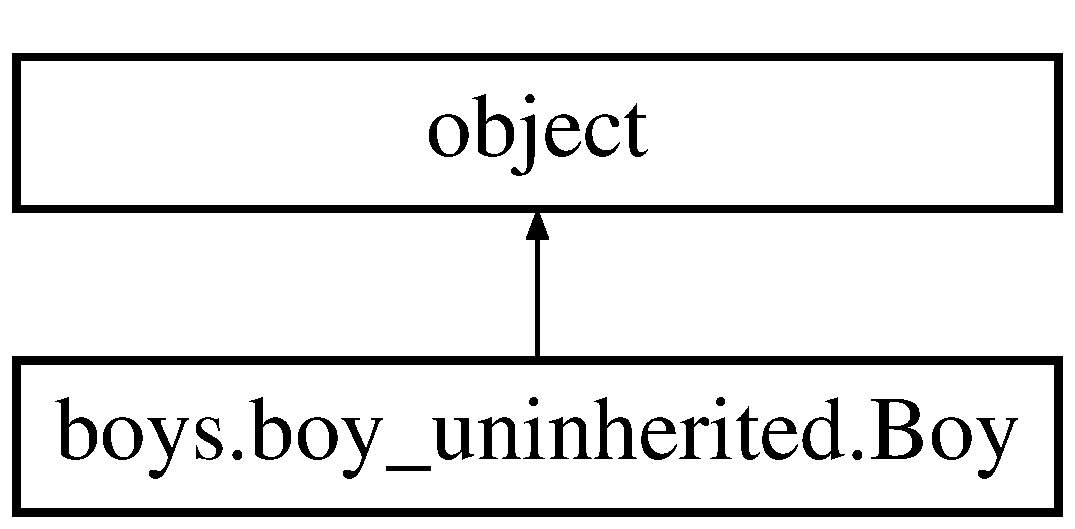
\includegraphics[height=2.000000cm]{classboys_1_1boy__uninherited_1_1_boy}
\end{center}
\end{figure}
\subsection*{Public Member Functions}
\begin{DoxyCompactItemize}
\item 
def \hyperlink{classboys_1_1boy__uninherited_1_1_boy_a0e3ae5ced04e7737f82917d5272860c0}{\+\_\+\+\_\+init\+\_\+\+\_\+} (self, \hyperlink{classboys_1_1boy__uninherited_1_1_boy_a4009413656c9d8057fc54545dce28df8}{name}, \hyperlink{classboys_1_1boy__uninherited_1_1_boy_afac2cde2111761c12ac48f3339f4c659}{attr}, \hyperlink{classboys_1_1boy__uninherited_1_1_boy_a0abd7cec036a08b7d7fb23db1709246d}{budget}, \hyperlink{classboys_1_1boy__uninherited_1_1_boy_a8069384d8d8dd16683ba292ac2b043b0}{intel}, \hyperlink{classboys_1_1boy__uninherited_1_1_boy_a95366dbf37df96f53c361a980791f4e7}{min\+\_\+attr}, \hyperlink{classboys_1_1boy__uninherited_1_1_boy_aea7eb7c4e32a8490a7280a8cb99f036d}{nature})
\item 
def \hyperlink{classboys_1_1boy__uninherited_1_1_boy_a833caeabdf27b25b3435776e01536b29}{check\+\_\+elligibility} (self, girl)
\item 
def \hyperlink{classboys_1_1boy__uninherited_1_1_boy_a1a8cc5381fb5b2fbd68698fc0791db97}{match} (self, girl)
\item 
def \hyperlink{classboys_1_1boy__uninherited_1_1_boy_a7a7071d13af4d9d43dd6a4eddbb4d55e}{set\+\_\+happiness} (self, gift\+\_\+basket)
\end{DoxyCompactItemize}
\subsection*{Public Attributes}
\begin{DoxyCompactItemize}
\item 
\hyperlink{classboys_1_1boy__uninherited_1_1_boy_a4009413656c9d8057fc54545dce28df8}{name}
\item 
\hyperlink{classboys_1_1boy__uninherited_1_1_boy_afac2cde2111761c12ac48f3339f4c659}{attr}
\item 
\hyperlink{classboys_1_1boy__uninherited_1_1_boy_a0abd7cec036a08b7d7fb23db1709246d}{budget}
\item 
\hyperlink{classboys_1_1boy__uninherited_1_1_boy_a8069384d8d8dd16683ba292ac2b043b0}{intel}
\item 
\hyperlink{classboys_1_1boy__uninherited_1_1_boy_a95366dbf37df96f53c361a980791f4e7}{min\+\_\+attr}
\item 
\hyperlink{classboys_1_1boy__uninherited_1_1_boy_a54bb9865e7dfb35e804b976d2d94a174}{status}
\item 
\hyperlink{classboys_1_1boy__uninherited_1_1_boy_aea7eb7c4e32a8490a7280a8cb99f036d}{nature}
\item 
\hyperlink{classboys_1_1boy__uninherited_1_1_boy_aa70bd494f431eff2fad089ac5ccf9403}{partner}
\item 
\hyperlink{classboys_1_1boy__uninherited_1_1_boy_a7de8536ac2f0ddaaf0dd4b7ffbba7e87}{happiness}
\end{DoxyCompactItemize}


\subsection{Detailed Description}
\begin{DoxyVerb}DOES NOT USE INHERITANCE\end{DoxyVerb}
 

\subsection{Constructor \& Destructor Documentation}
\index{boys\+::boy\+\_\+uninherited\+::\+Boy@{boys\+::boy\+\_\+uninherited\+::\+Boy}!\+\_\+\+\_\+init\+\_\+\+\_\+@{\+\_\+\+\_\+init\+\_\+\+\_\+}}
\index{\+\_\+\+\_\+init\+\_\+\+\_\+@{\+\_\+\+\_\+init\+\_\+\+\_\+}!boys\+::boy\+\_\+uninherited\+::\+Boy@{boys\+::boy\+\_\+uninherited\+::\+Boy}}
\subsubsection[{\texorpdfstring{\+\_\+\+\_\+init\+\_\+\+\_\+(self, name, attr, budget, intel, min\+\_\+attr, nature)}{__init__(self, name, attr, budget, intel, min_attr, nature)}}]{\setlength{\rightskip}{0pt plus 5cm}def boys.\+boy\+\_\+uninherited.\+Boy.\+\_\+\+\_\+init\+\_\+\+\_\+ (
\begin{DoxyParamCaption}
\item[{}]{self, }
\item[{}]{name, }
\item[{}]{attr, }
\item[{}]{budget, }
\item[{}]{intel, }
\item[{}]{min\+\_\+attr, }
\item[{}]{nature}
\end{DoxyParamCaption}
)}\hypertarget{classboys_1_1boy__uninherited_1_1_boy_a0e3ae5ced04e7737f82917d5272860c0}{}\label{classboys_1_1boy__uninherited_1_1_boy_a0e3ae5ced04e7737f82917d5272860c0}
\begin{DoxyVerb}DEFAULT CONSTRUCTOR\end{DoxyVerb}
 

\subsection{Member Function Documentation}
\index{boys\+::boy\+\_\+uninherited\+::\+Boy@{boys\+::boy\+\_\+uninherited\+::\+Boy}!check\+\_\+elligibility@{check\+\_\+elligibility}}
\index{check\+\_\+elligibility@{check\+\_\+elligibility}!boys\+::boy\+\_\+uninherited\+::\+Boy@{boys\+::boy\+\_\+uninherited\+::\+Boy}}
\subsubsection[{\texorpdfstring{check\+\_\+elligibility(self, girl)}{check_elligibility(self, girl)}}]{\setlength{\rightskip}{0pt plus 5cm}def boys.\+boy\+\_\+uninherited.\+Boy.\+check\+\_\+elligibility (
\begin{DoxyParamCaption}
\item[{}]{self, }
\item[{}]{girl}
\end{DoxyParamCaption}
)}\hypertarget{classboys_1_1boy__uninherited_1_1_boy_a833caeabdf27b25b3435776e01536b29}{}\label{classboys_1_1boy__uninherited_1_1_boy_a833caeabdf27b25b3435776e01536b29}
\begin{DoxyVerb}CHECKS WHETHER THIS BOY IS ELIGIBLE FOR PAIRING WITH THE CURRENT GIRL\end{DoxyVerb}
 \index{boys\+::boy\+\_\+uninherited\+::\+Boy@{boys\+::boy\+\_\+uninherited\+::\+Boy}!match@{match}}
\index{match@{match}!boys\+::boy\+\_\+uninherited\+::\+Boy@{boys\+::boy\+\_\+uninherited\+::\+Boy}}
\subsubsection[{\texorpdfstring{match(self, girl)}{match(self, girl)}}]{\setlength{\rightskip}{0pt plus 5cm}def boys.\+boy\+\_\+uninherited.\+Boy.\+match (
\begin{DoxyParamCaption}
\item[{}]{self, }
\item[{}]{girl}
\end{DoxyParamCaption}
)}\hypertarget{classboys_1_1boy__uninherited_1_1_boy_a1a8cc5381fb5b2fbd68698fc0791db97}{}\label{classboys_1_1boy__uninherited_1_1_boy_a1a8cc5381fb5b2fbd68698fc0791db97}
\begin{DoxyVerb}ASSIGNS GIRL AS THE PARTNER FOR THIS BOY\end{DoxyVerb}
 \index{boys\+::boy\+\_\+uninherited\+::\+Boy@{boys\+::boy\+\_\+uninherited\+::\+Boy}!set\+\_\+happiness@{set\+\_\+happiness}}
\index{set\+\_\+happiness@{set\+\_\+happiness}!boys\+::boy\+\_\+uninherited\+::\+Boy@{boys\+::boy\+\_\+uninherited\+::\+Boy}}
\subsubsection[{\texorpdfstring{set\+\_\+happiness(self, gift\+\_\+basket)}{set_happiness(self, gift_basket)}}]{\setlength{\rightskip}{0pt plus 5cm}def boys.\+boy\+\_\+uninherited.\+Boy.\+set\+\_\+happiness (
\begin{DoxyParamCaption}
\item[{}]{self, }
\item[{}]{gift\+\_\+basket}
\end{DoxyParamCaption}
)}\hypertarget{classboys_1_1boy__uninherited_1_1_boy_a7a7071d13af4d9d43dd6a4eddbb4d55e}{}\label{classboys_1_1boy__uninherited_1_1_boy_a7a7071d13af4d9d43dd6a4eddbb4d55e}
\begin{DoxyVerb}CALCULATES HAPPINESS OF THIS BOY\end{DoxyVerb}
 

\subsection{Member Data Documentation}
\index{boys\+::boy\+\_\+uninherited\+::\+Boy@{boys\+::boy\+\_\+uninherited\+::\+Boy}!attr@{attr}}
\index{attr@{attr}!boys\+::boy\+\_\+uninherited\+::\+Boy@{boys\+::boy\+\_\+uninherited\+::\+Boy}}
\subsubsection[{\texorpdfstring{attr}{attr}}]{\setlength{\rightskip}{0pt plus 5cm}boys.\+boy\+\_\+uninherited.\+Boy.\+attr}\hypertarget{classboys_1_1boy__uninherited_1_1_boy_afac2cde2111761c12ac48f3339f4c659}{}\label{classboys_1_1boy__uninherited_1_1_boy_afac2cde2111761c12ac48f3339f4c659}
\index{boys\+::boy\+\_\+uninherited\+::\+Boy@{boys\+::boy\+\_\+uninherited\+::\+Boy}!budget@{budget}}
\index{budget@{budget}!boys\+::boy\+\_\+uninherited\+::\+Boy@{boys\+::boy\+\_\+uninherited\+::\+Boy}}
\subsubsection[{\texorpdfstring{budget}{budget}}]{\setlength{\rightskip}{0pt plus 5cm}boys.\+boy\+\_\+uninherited.\+Boy.\+budget}\hypertarget{classboys_1_1boy__uninherited_1_1_boy_a0abd7cec036a08b7d7fb23db1709246d}{}\label{classboys_1_1boy__uninherited_1_1_boy_a0abd7cec036a08b7d7fb23db1709246d}
\index{boys\+::boy\+\_\+uninherited\+::\+Boy@{boys\+::boy\+\_\+uninherited\+::\+Boy}!happiness@{happiness}}
\index{happiness@{happiness}!boys\+::boy\+\_\+uninherited\+::\+Boy@{boys\+::boy\+\_\+uninherited\+::\+Boy}}
\subsubsection[{\texorpdfstring{happiness}{happiness}}]{\setlength{\rightskip}{0pt plus 5cm}boys.\+boy\+\_\+uninherited.\+Boy.\+happiness}\hypertarget{classboys_1_1boy__uninherited_1_1_boy_a7de8536ac2f0ddaaf0dd4b7ffbba7e87}{}\label{classboys_1_1boy__uninherited_1_1_boy_a7de8536ac2f0ddaaf0dd4b7ffbba7e87}
\index{boys\+::boy\+\_\+uninherited\+::\+Boy@{boys\+::boy\+\_\+uninherited\+::\+Boy}!intel@{intel}}
\index{intel@{intel}!boys\+::boy\+\_\+uninherited\+::\+Boy@{boys\+::boy\+\_\+uninherited\+::\+Boy}}
\subsubsection[{\texorpdfstring{intel}{intel}}]{\setlength{\rightskip}{0pt plus 5cm}boys.\+boy\+\_\+uninherited.\+Boy.\+intel}\hypertarget{classboys_1_1boy__uninherited_1_1_boy_a8069384d8d8dd16683ba292ac2b043b0}{}\label{classboys_1_1boy__uninherited_1_1_boy_a8069384d8d8dd16683ba292ac2b043b0}
\index{boys\+::boy\+\_\+uninherited\+::\+Boy@{boys\+::boy\+\_\+uninherited\+::\+Boy}!min\+\_\+attr@{min\+\_\+attr}}
\index{min\+\_\+attr@{min\+\_\+attr}!boys\+::boy\+\_\+uninherited\+::\+Boy@{boys\+::boy\+\_\+uninherited\+::\+Boy}}
\subsubsection[{\texorpdfstring{min\+\_\+attr}{min_attr}}]{\setlength{\rightskip}{0pt plus 5cm}boys.\+boy\+\_\+uninherited.\+Boy.\+min\+\_\+attr}\hypertarget{classboys_1_1boy__uninherited_1_1_boy_a95366dbf37df96f53c361a980791f4e7}{}\label{classboys_1_1boy__uninherited_1_1_boy_a95366dbf37df96f53c361a980791f4e7}
\index{boys\+::boy\+\_\+uninherited\+::\+Boy@{boys\+::boy\+\_\+uninherited\+::\+Boy}!name@{name}}
\index{name@{name}!boys\+::boy\+\_\+uninherited\+::\+Boy@{boys\+::boy\+\_\+uninherited\+::\+Boy}}
\subsubsection[{\texorpdfstring{name}{name}}]{\setlength{\rightskip}{0pt plus 5cm}boys.\+boy\+\_\+uninherited.\+Boy.\+name}\hypertarget{classboys_1_1boy__uninherited_1_1_boy_a4009413656c9d8057fc54545dce28df8}{}\label{classboys_1_1boy__uninherited_1_1_boy_a4009413656c9d8057fc54545dce28df8}
\index{boys\+::boy\+\_\+uninherited\+::\+Boy@{boys\+::boy\+\_\+uninherited\+::\+Boy}!nature@{nature}}
\index{nature@{nature}!boys\+::boy\+\_\+uninherited\+::\+Boy@{boys\+::boy\+\_\+uninherited\+::\+Boy}}
\subsubsection[{\texorpdfstring{nature}{nature}}]{\setlength{\rightskip}{0pt plus 5cm}boys.\+boy\+\_\+uninherited.\+Boy.\+nature}\hypertarget{classboys_1_1boy__uninherited_1_1_boy_aea7eb7c4e32a8490a7280a8cb99f036d}{}\label{classboys_1_1boy__uninherited_1_1_boy_aea7eb7c4e32a8490a7280a8cb99f036d}
\index{boys\+::boy\+\_\+uninherited\+::\+Boy@{boys\+::boy\+\_\+uninherited\+::\+Boy}!partner@{partner}}
\index{partner@{partner}!boys\+::boy\+\_\+uninherited\+::\+Boy@{boys\+::boy\+\_\+uninherited\+::\+Boy}}
\subsubsection[{\texorpdfstring{partner}{partner}}]{\setlength{\rightskip}{0pt plus 5cm}boys.\+boy\+\_\+uninherited.\+Boy.\+partner}\hypertarget{classboys_1_1boy__uninherited_1_1_boy_aa70bd494f431eff2fad089ac5ccf9403}{}\label{classboys_1_1boy__uninherited_1_1_boy_aa70bd494f431eff2fad089ac5ccf9403}
\index{boys\+::boy\+\_\+uninherited\+::\+Boy@{boys\+::boy\+\_\+uninherited\+::\+Boy}!status@{status}}
\index{status@{status}!boys\+::boy\+\_\+uninherited\+::\+Boy@{boys\+::boy\+\_\+uninherited\+::\+Boy}}
\subsubsection[{\texorpdfstring{status}{status}}]{\setlength{\rightskip}{0pt plus 5cm}boys.\+boy\+\_\+uninherited.\+Boy.\+status}\hypertarget{classboys_1_1boy__uninherited_1_1_boy_a54bb9865e7dfb35e804b976d2d94a174}{}\label{classboys_1_1boy__uninherited_1_1_boy_a54bb9865e7dfb35e804b976d2d94a174}


The documentation for this class was generated from the following file\+:\begin{DoxyCompactItemize}
\item 
/media/illuminatus/\+Study/\+Python Programming/\+Projects/\+P\+P\+L Assignment/boys/\hyperlink{boy__uninherited_8py}{boy\+\_\+uninherited.\+py}\end{DoxyCompactItemize}

\hypertarget{classcouple_1_1_couple}{}\section{couple.\+Couple Class Reference}
\label{classcouple_1_1_couple}\index{couple.\+Couple@{couple.\+Couple}}


Inheritance diagram for couple.\+Couple\+:
\nopagebreak
\begin{figure}[H]
\begin{center}
\leavevmode
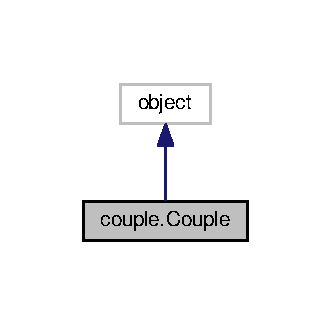
\includegraphics[width=159pt]{classcouple_1_1_couple__inherit__graph}
\end{center}
\end{figure}


Collaboration diagram for couple.\+Couple\+:
\nopagebreak
\begin{figure}[H]
\begin{center}
\leavevmode
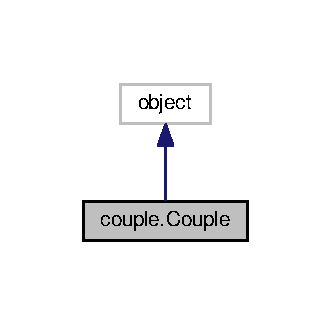
\includegraphics[width=159pt]{classcouple_1_1_couple__coll__graph}
\end{center}
\end{figure}
\subsection*{Public Member Functions}
\begin{DoxyCompactItemize}
\item 
def \hyperlink{classcouple_1_1_couple_a3cd6b67c48b545c1b51a8c11ac70677c}{\+\_\+\+\_\+init\+\_\+\+\_\+} (self, \hyperlink{classcouple_1_1_couple_a9add8e4c50bcbf4424339df43ed77df6}{boy}, \hyperlink{classcouple_1_1_couple_a99b4aa0aa5cd56aab0edebbba13e31b3}{girl})
\item 
def \hyperlink{classcouple_1_1_couple_a98db0e4bc5aa8bc81c3f5a2b05167c5f}{set\+\_\+happiness} (self)
\item 
def \hyperlink{classcouple_1_1_couple_a6557f9a740d1fc4750f3350e8138b0db}{set\+\_\+compatibility} (self)
\end{DoxyCompactItemize}
\subsection*{Public Attributes}
\begin{DoxyCompactItemize}
\item 
\hyperlink{classcouple_1_1_couple_a9add8e4c50bcbf4424339df43ed77df6}{boy}
\item 
\hyperlink{classcouple_1_1_couple_a99b4aa0aa5cd56aab0edebbba13e31b3}{girl}
\item 
\hyperlink{classcouple_1_1_couple_acfd8db3febb395596db4f5ab4ed53976}{happiness}
\item 
\hyperlink{classcouple_1_1_couple_a1b040704af8f391cacef5d15ef602717}{compatibility}
\item 
\hyperlink{classcouple_1_1_couple_a9cc14db20e8558bf7927df38789529a2}{gift\+\_\+basket}
\end{DoxyCompactItemize}


\subsection{Detailed Description}
\begin{DoxyVerb}COUPLE CLASS\end{DoxyVerb}
 

Definition at line 3 of file couple.\+py.



\subsection{Constructor \& Destructor Documentation}
\index{couple\+::\+Couple@{couple\+::\+Couple}!\+\_\+\+\_\+init\+\_\+\+\_\+@{\+\_\+\+\_\+init\+\_\+\+\_\+}}
\index{\+\_\+\+\_\+init\+\_\+\+\_\+@{\+\_\+\+\_\+init\+\_\+\+\_\+}!couple\+::\+Couple@{couple\+::\+Couple}}
\subsubsection[{\texorpdfstring{\+\_\+\+\_\+init\+\_\+\+\_\+(self, boy, girl)}{__init__(self, boy, girl)}}]{\setlength{\rightskip}{0pt plus 5cm}def couple.\+Couple.\+\_\+\+\_\+init\+\_\+\+\_\+ (
\begin{DoxyParamCaption}
\item[{}]{self, }
\item[{}]{boy, }
\item[{}]{girl}
\end{DoxyParamCaption}
)}\hypertarget{classcouple_1_1_couple_a3cd6b67c48b545c1b51a8c11ac70677c}{}\label{classcouple_1_1_couple_a3cd6b67c48b545c1b51a8c11ac70677c}
\begin{DoxyVerb}DEFAULT CONSTRUCTOR\end{DoxyVerb}
 

Definition at line 7 of file couple.\+py.



\subsection{Member Function Documentation}
\index{couple\+::\+Couple@{couple\+::\+Couple}!set\+\_\+compatibility@{set\+\_\+compatibility}}
\index{set\+\_\+compatibility@{set\+\_\+compatibility}!couple\+::\+Couple@{couple\+::\+Couple}}
\subsubsection[{\texorpdfstring{set\+\_\+compatibility(self)}{set_compatibility(self)}}]{\setlength{\rightskip}{0pt plus 5cm}def couple.\+Couple.\+set\+\_\+compatibility (
\begin{DoxyParamCaption}
\item[{}]{self}
\end{DoxyParamCaption}
)}\hypertarget{classcouple_1_1_couple_a6557f9a740d1fc4750f3350e8138b0db}{}\label{classcouple_1_1_couple_a6557f9a740d1fc4750f3350e8138b0db}
\begin{DoxyVerb}CALCULATES COUPLE'S COMPATIBILITY\end{DoxyVerb}
 

Definition at line 19 of file couple.\+py.

\index{couple\+::\+Couple@{couple\+::\+Couple}!set\+\_\+happiness@{set\+\_\+happiness}}
\index{set\+\_\+happiness@{set\+\_\+happiness}!couple\+::\+Couple@{couple\+::\+Couple}}
\subsubsection[{\texorpdfstring{set\+\_\+happiness(self)}{set_happiness(self)}}]{\setlength{\rightskip}{0pt plus 5cm}def couple.\+Couple.\+set\+\_\+happiness (
\begin{DoxyParamCaption}
\item[{}]{self}
\end{DoxyParamCaption}
)}\hypertarget{classcouple_1_1_couple_a98db0e4bc5aa8bc81c3f5a2b05167c5f}{}\label{classcouple_1_1_couple_a98db0e4bc5aa8bc81c3f5a2b05167c5f}
\begin{DoxyVerb}CALCULATES COUPLE'S HAPPINESS\end{DoxyVerb}
 

Definition at line 15 of file couple.\+py.



\subsection{Member Data Documentation}
\index{couple\+::\+Couple@{couple\+::\+Couple}!boy@{boy}}
\index{boy@{boy}!couple\+::\+Couple@{couple\+::\+Couple}}
\subsubsection[{\texorpdfstring{boy}{boy}}]{\setlength{\rightskip}{0pt plus 5cm}couple.\+Couple.\+boy}\hypertarget{classcouple_1_1_couple_a9add8e4c50bcbf4424339df43ed77df6}{}\label{classcouple_1_1_couple_a9add8e4c50bcbf4424339df43ed77df6}


Definition at line 9 of file couple.\+py.

\index{couple\+::\+Couple@{couple\+::\+Couple}!compatibility@{compatibility}}
\index{compatibility@{compatibility}!couple\+::\+Couple@{couple\+::\+Couple}}
\subsubsection[{\texorpdfstring{compatibility}{compatibility}}]{\setlength{\rightskip}{0pt plus 5cm}couple.\+Couple.\+compatibility}\hypertarget{classcouple_1_1_couple_a1b040704af8f391cacef5d15ef602717}{}\label{classcouple_1_1_couple_a1b040704af8f391cacef5d15ef602717}


Definition at line 12 of file couple.\+py.

\index{couple\+::\+Couple@{couple\+::\+Couple}!gift\+\_\+basket@{gift\+\_\+basket}}
\index{gift\+\_\+basket@{gift\+\_\+basket}!couple\+::\+Couple@{couple\+::\+Couple}}
\subsubsection[{\texorpdfstring{gift\+\_\+basket}{gift_basket}}]{\setlength{\rightskip}{0pt plus 5cm}couple.\+Couple.\+gift\+\_\+basket}\hypertarget{classcouple_1_1_couple_a9cc14db20e8558bf7927df38789529a2}{}\label{classcouple_1_1_couple_a9cc14db20e8558bf7927df38789529a2}


Definition at line 13 of file couple.\+py.

\index{couple\+::\+Couple@{couple\+::\+Couple}!girl@{girl}}
\index{girl@{girl}!couple\+::\+Couple@{couple\+::\+Couple}}
\subsubsection[{\texorpdfstring{girl}{girl}}]{\setlength{\rightskip}{0pt plus 5cm}couple.\+Couple.\+girl}\hypertarget{classcouple_1_1_couple_a99b4aa0aa5cd56aab0edebbba13e31b3}{}\label{classcouple_1_1_couple_a99b4aa0aa5cd56aab0edebbba13e31b3}


Definition at line 10 of file couple.\+py.

\index{couple\+::\+Couple@{couple\+::\+Couple}!happiness@{happiness}}
\index{happiness@{happiness}!couple\+::\+Couple@{couple\+::\+Couple}}
\subsubsection[{\texorpdfstring{happiness}{happiness}}]{\setlength{\rightskip}{0pt plus 5cm}couple.\+Couple.\+happiness}\hypertarget{classcouple_1_1_couple_acfd8db3febb395596db4f5ab4ed53976}{}\label{classcouple_1_1_couple_acfd8db3febb395596db4f5ab4ed53976}


Definition at line 11 of file couple.\+py.



The documentation for this class was generated from the following file\+:\begin{DoxyCompactItemize}
\item 
/media/illuminatus/\+Study/\+Python Programming/\+Projects/\+P\+P\+L Assignment/\hyperlink{couple_8py}{couple.\+py}\end{DoxyCompactItemize}

\hypertarget{classgifts_1_1gift__uninherited_1_1_gift}{}\section{gifts.\+gift\+\_\+uninherited.\+Gift Class Reference}
\label{classgifts_1_1gift__uninherited_1_1_gift}\index{gifts.\+gift\+\_\+uninherited.\+Gift@{gifts.\+gift\+\_\+uninherited.\+Gift}}


Inheritance diagram for gifts.\+gift\+\_\+uninherited.\+Gift\+:
\nopagebreak
\begin{figure}[H]
\begin{center}
\leavevmode
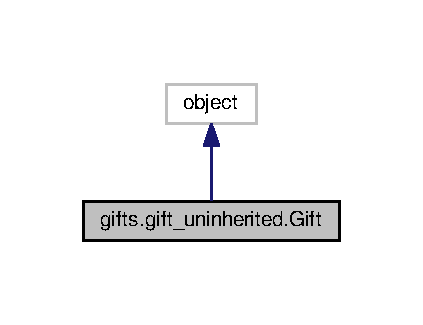
\includegraphics[width=203pt]{classgifts_1_1gift__uninherited_1_1_gift__inherit__graph}
\end{center}
\end{figure}


Collaboration diagram for gifts.\+gift\+\_\+uninherited.\+Gift\+:
\nopagebreak
\begin{figure}[H]
\begin{center}
\leavevmode
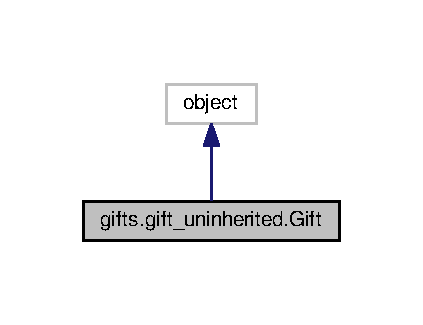
\includegraphics[width=203pt]{classgifts_1_1gift__uninherited_1_1_gift__coll__graph}
\end{center}
\end{figure}
\subsection*{Public Member Functions}
\begin{DoxyCompactItemize}
\item 
def \hyperlink{classgifts_1_1gift__uninherited_1_1_gift_a78eaebfe6b720d93b8ae2d475a6dd613}{\+\_\+\+\_\+init\+\_\+\+\_\+} (self, \hyperlink{classgifts_1_1gift__uninherited_1_1_gift_abe76c25355d683ddd1e2383f139e4f8e}{name}, \hyperlink{classgifts_1_1gift__uninherited_1_1_gift_a0f92afe5566c82745e3b3759d2e9f775}{price}, \hyperlink{classgifts_1_1gift__uninherited_1_1_gift_aea65e2d06b96ec3ab267e4e8dd1e91ff}{value}, \hyperlink{classgifts_1_1gift__uninherited_1_1_gift_ac21294038fa6ce0cd1a192e303fc1920}{nature}, \hyperlink{classgifts_1_1gift__uninherited_1_1_gift_ae4594046255e648f0496354d1eb540ce}{rating}, \hyperlink{classgifts_1_1gift__uninherited_1_1_gift_ae679bef0b9d26aad227c52602b8575ee}{difficulty}, \hyperlink{classgifts_1_1gift__uninherited_1_1_gift_a640df8d6eb45f9027260eb8053bb6b43}{util\+\_\+value}, \hyperlink{classgifts_1_1gift__uninherited_1_1_gift_a7fd2164d8bd791fa524e82d2ef6316aa}{util\+\_\+class})
\end{DoxyCompactItemize}
\subsection*{Public Attributes}
\begin{DoxyCompactItemize}
\item 
\hyperlink{classgifts_1_1gift__uninherited_1_1_gift_abe76c25355d683ddd1e2383f139e4f8e}{name}
\item 
\hyperlink{classgifts_1_1gift__uninherited_1_1_gift_a0f92afe5566c82745e3b3759d2e9f775}{price}
\item 
\hyperlink{classgifts_1_1gift__uninherited_1_1_gift_aea65e2d06b96ec3ab267e4e8dd1e91ff}{value}
\item 
\hyperlink{classgifts_1_1gift__uninherited_1_1_gift_ac21294038fa6ce0cd1a192e303fc1920}{nature}
\item 
\hyperlink{classgifts_1_1gift__uninherited_1_1_gift_ae4594046255e648f0496354d1eb540ce}{rating}
\item 
\hyperlink{classgifts_1_1gift__uninherited_1_1_gift_ae679bef0b9d26aad227c52602b8575ee}{difficulty}
\item 
\hyperlink{classgifts_1_1gift__uninherited_1_1_gift_a640df8d6eb45f9027260eb8053bb6b43}{util\+\_\+value}
\item 
\hyperlink{classgifts_1_1gift__uninherited_1_1_gift_a7fd2164d8bd791fa524e82d2ef6316aa}{util\+\_\+class}
\end{DoxyCompactItemize}


\subsection{Detailed Description}
\begin{DoxyVerb}DOES NOT USE INHERITANCE\end{DoxyVerb}
 

Definition at line 3 of file gift\+\_\+uninherited.\+py.



\subsection{Constructor \& Destructor Documentation}
\index{gifts\+::gift\+\_\+uninherited\+::\+Gift@{gifts\+::gift\+\_\+uninherited\+::\+Gift}!\+\_\+\+\_\+init\+\_\+\+\_\+@{\+\_\+\+\_\+init\+\_\+\+\_\+}}
\index{\+\_\+\+\_\+init\+\_\+\+\_\+@{\+\_\+\+\_\+init\+\_\+\+\_\+}!gifts\+::gift\+\_\+uninherited\+::\+Gift@{gifts\+::gift\+\_\+uninherited\+::\+Gift}}
\subsubsection[{\texorpdfstring{\+\_\+\+\_\+init\+\_\+\+\_\+(self, name, price, value, nature, rating, difficulty, util\+\_\+value, util\+\_\+class)}{__init__(self, name, price, value, nature, rating, difficulty, util_value, util_class)}}]{\setlength{\rightskip}{0pt plus 5cm}def gifts.\+gift\+\_\+uninherited.\+Gift.\+\_\+\+\_\+init\+\_\+\+\_\+ (
\begin{DoxyParamCaption}
\item[{}]{self, }
\item[{}]{name, }
\item[{}]{price, }
\item[{}]{value, }
\item[{}]{nature, }
\item[{}]{rating, }
\item[{}]{difficulty, }
\item[{}]{util\+\_\+value, }
\item[{}]{util\+\_\+class}
\end{DoxyParamCaption}
)}\hypertarget{classgifts_1_1gift__uninherited_1_1_gift_a78eaebfe6b720d93b8ae2d475a6dd613}{}\label{classgifts_1_1gift__uninherited_1_1_gift_a78eaebfe6b720d93b8ae2d475a6dd613}
\begin{DoxyVerb}DEFAULT CONSTRUCTOR\end{DoxyVerb}
 

Definition at line 7 of file gift\+\_\+uninherited.\+py.



\subsection{Member Data Documentation}
\index{gifts\+::gift\+\_\+uninherited\+::\+Gift@{gifts\+::gift\+\_\+uninherited\+::\+Gift}!difficulty@{difficulty}}
\index{difficulty@{difficulty}!gifts\+::gift\+\_\+uninherited\+::\+Gift@{gifts\+::gift\+\_\+uninherited\+::\+Gift}}
\subsubsection[{\texorpdfstring{difficulty}{difficulty}}]{\setlength{\rightskip}{0pt plus 5cm}gifts.\+gift\+\_\+uninherited.\+Gift.\+difficulty}\hypertarget{classgifts_1_1gift__uninherited_1_1_gift_ae679bef0b9d26aad227c52602b8575ee}{}\label{classgifts_1_1gift__uninherited_1_1_gift_ae679bef0b9d26aad227c52602b8575ee}


Definition at line 16 of file gift\+\_\+uninherited.\+py.

\index{gifts\+::gift\+\_\+uninherited\+::\+Gift@{gifts\+::gift\+\_\+uninherited\+::\+Gift}!name@{name}}
\index{name@{name}!gifts\+::gift\+\_\+uninherited\+::\+Gift@{gifts\+::gift\+\_\+uninherited\+::\+Gift}}
\subsubsection[{\texorpdfstring{name}{name}}]{\setlength{\rightskip}{0pt plus 5cm}gifts.\+gift\+\_\+uninherited.\+Gift.\+name}\hypertarget{classgifts_1_1gift__uninherited_1_1_gift_abe76c25355d683ddd1e2383f139e4f8e}{}\label{classgifts_1_1gift__uninherited_1_1_gift_abe76c25355d683ddd1e2383f139e4f8e}


Definition at line 9 of file gift\+\_\+uninherited.\+py.

\index{gifts\+::gift\+\_\+uninherited\+::\+Gift@{gifts\+::gift\+\_\+uninherited\+::\+Gift}!nature@{nature}}
\index{nature@{nature}!gifts\+::gift\+\_\+uninherited\+::\+Gift@{gifts\+::gift\+\_\+uninherited\+::\+Gift}}
\subsubsection[{\texorpdfstring{nature}{nature}}]{\setlength{\rightskip}{0pt plus 5cm}gifts.\+gift\+\_\+uninherited.\+Gift.\+nature}\hypertarget{classgifts_1_1gift__uninherited_1_1_gift_ac21294038fa6ce0cd1a192e303fc1920}{}\label{classgifts_1_1gift__uninherited_1_1_gift_ac21294038fa6ce0cd1a192e303fc1920}


Definition at line 12 of file gift\+\_\+uninherited.\+py.

\index{gifts\+::gift\+\_\+uninherited\+::\+Gift@{gifts\+::gift\+\_\+uninherited\+::\+Gift}!price@{price}}
\index{price@{price}!gifts\+::gift\+\_\+uninherited\+::\+Gift@{gifts\+::gift\+\_\+uninherited\+::\+Gift}}
\subsubsection[{\texorpdfstring{price}{price}}]{\setlength{\rightskip}{0pt plus 5cm}gifts.\+gift\+\_\+uninherited.\+Gift.\+price}\hypertarget{classgifts_1_1gift__uninherited_1_1_gift_a0f92afe5566c82745e3b3759d2e9f775}{}\label{classgifts_1_1gift__uninherited_1_1_gift_a0f92afe5566c82745e3b3759d2e9f775}


Definition at line 10 of file gift\+\_\+uninherited.\+py.

\index{gifts\+::gift\+\_\+uninherited\+::\+Gift@{gifts\+::gift\+\_\+uninherited\+::\+Gift}!rating@{rating}}
\index{rating@{rating}!gifts\+::gift\+\_\+uninherited\+::\+Gift@{gifts\+::gift\+\_\+uninherited\+::\+Gift}}
\subsubsection[{\texorpdfstring{rating}{rating}}]{\setlength{\rightskip}{0pt plus 5cm}gifts.\+gift\+\_\+uninherited.\+Gift.\+rating}\hypertarget{classgifts_1_1gift__uninherited_1_1_gift_ae4594046255e648f0496354d1eb540ce}{}\label{classgifts_1_1gift__uninherited_1_1_gift_ae4594046255e648f0496354d1eb540ce}


Definition at line 15 of file gift\+\_\+uninherited.\+py.

\index{gifts\+::gift\+\_\+uninherited\+::\+Gift@{gifts\+::gift\+\_\+uninherited\+::\+Gift}!util\+\_\+class@{util\+\_\+class}}
\index{util\+\_\+class@{util\+\_\+class}!gifts\+::gift\+\_\+uninherited\+::\+Gift@{gifts\+::gift\+\_\+uninherited\+::\+Gift}}
\subsubsection[{\texorpdfstring{util\+\_\+class}{util_class}}]{\setlength{\rightskip}{0pt plus 5cm}gifts.\+gift\+\_\+uninherited.\+Gift.\+util\+\_\+class}\hypertarget{classgifts_1_1gift__uninherited_1_1_gift_a7fd2164d8bd791fa524e82d2ef6316aa}{}\label{classgifts_1_1gift__uninherited_1_1_gift_a7fd2164d8bd791fa524e82d2ef6316aa}


Definition at line 20 of file gift\+\_\+uninherited.\+py.

\index{gifts\+::gift\+\_\+uninherited\+::\+Gift@{gifts\+::gift\+\_\+uninherited\+::\+Gift}!util\+\_\+value@{util\+\_\+value}}
\index{util\+\_\+value@{util\+\_\+value}!gifts\+::gift\+\_\+uninherited\+::\+Gift@{gifts\+::gift\+\_\+uninherited\+::\+Gift}}
\subsubsection[{\texorpdfstring{util\+\_\+value}{util_value}}]{\setlength{\rightskip}{0pt plus 5cm}gifts.\+gift\+\_\+uninherited.\+Gift.\+util\+\_\+value}\hypertarget{classgifts_1_1gift__uninherited_1_1_gift_a640df8d6eb45f9027260eb8053bb6b43}{}\label{classgifts_1_1gift__uninherited_1_1_gift_a640df8d6eb45f9027260eb8053bb6b43}


Definition at line 19 of file gift\+\_\+uninherited.\+py.

\index{gifts\+::gift\+\_\+uninherited\+::\+Gift@{gifts\+::gift\+\_\+uninherited\+::\+Gift}!value@{value}}
\index{value@{value}!gifts\+::gift\+\_\+uninherited\+::\+Gift@{gifts\+::gift\+\_\+uninherited\+::\+Gift}}
\subsubsection[{\texorpdfstring{value}{value}}]{\setlength{\rightskip}{0pt plus 5cm}gifts.\+gift\+\_\+uninherited.\+Gift.\+value}\hypertarget{classgifts_1_1gift__uninherited_1_1_gift_aea65e2d06b96ec3ab267e4e8dd1e91ff}{}\label{classgifts_1_1gift__uninherited_1_1_gift_aea65e2d06b96ec3ab267e4e8dd1e91ff}


Definition at line 11 of file gift\+\_\+uninherited.\+py.



The documentation for this class was generated from the following file\+:\begin{DoxyCompactItemize}
\item 
/media/illuminatus/\+Study/\+Python Programming/\+Projects/\+P\+P\+L Assignment/gifts/\hyperlink{gift__uninherited_8py}{gift\+\_\+uninherited.\+py}\end{DoxyCompactItemize}

\hypertarget{classgirls_1_1girl__uninherited_1_1_girl}{}\section{girls.\+girl\+\_\+uninherited.\+Girl Class Reference}
\label{classgirls_1_1girl__uninherited_1_1_girl}\index{girls.\+girl\+\_\+uninherited.\+Girl@{girls.\+girl\+\_\+uninherited.\+Girl}}
Inheritance diagram for girls.\+girl\+\_\+uninherited.\+Girl\+:\begin{figure}[H]
\begin{center}
\leavevmode
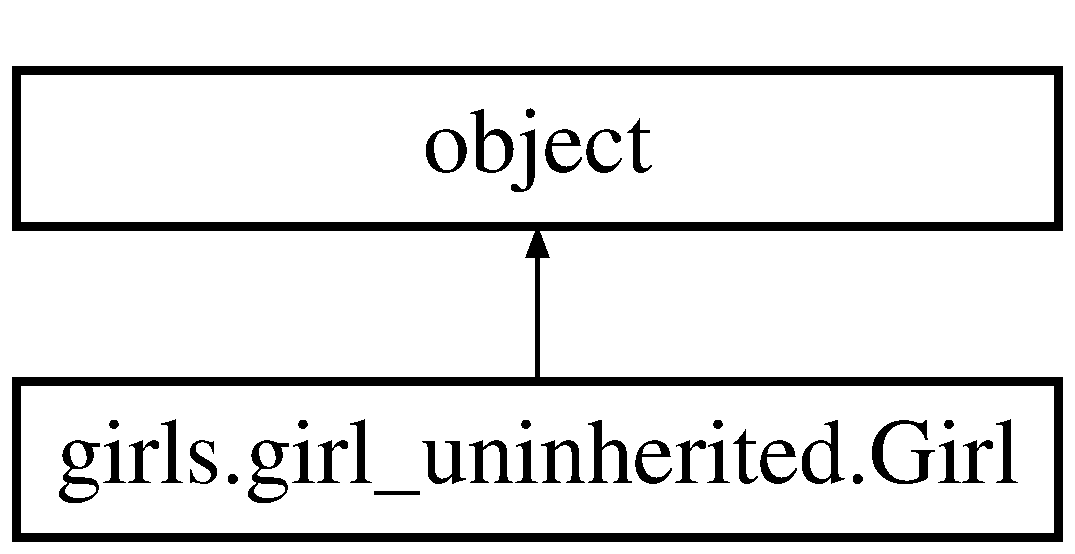
\includegraphics[height=2.000000cm]{classgirls_1_1girl__uninherited_1_1_girl}
\end{center}
\end{figure}
\subsection*{Public Member Functions}
\begin{DoxyCompactItemize}
\item 
def \hyperlink{classgirls_1_1girl__uninherited_1_1_girl_a3baf6cbbda021313abf57a4b2d2e9efa}{\+\_\+\+\_\+init\+\_\+\+\_\+} (self, \hyperlink{classgirls_1_1girl__uninherited_1_1_girl_a17de9450938ef15ad772de7a1acfc197}{name}, \hyperlink{classgirls_1_1girl__uninherited_1_1_girl_a3f915cb51744e34e3d2f88624b402148}{attr}, \hyperlink{classgirls_1_1girl__uninherited_1_1_girl_a6a34ca1b5efd14cc0c70e2a0bd0202dc}{mcost}, \hyperlink{classgirls_1_1girl__uninherited_1_1_girl_a820d0a86b6f84b7d3fc75d142cdedfdc}{intel}, \hyperlink{classgirls_1_1girl__uninherited_1_1_girl_af4b8bfdd9e572a69ce4f5bd047fe4aad}{nature}, \hyperlink{classgirls_1_1girl__uninherited_1_1_girl_a35076aa934b12cc39ae778cf0bb176c9}{criteria})
\item 
def \hyperlink{classgirls_1_1girl__uninherited_1_1_girl_a0fd44810c87eaef7df92c264d5b8f864}{check\+\_\+elligibility} (self, boy)
\item 
def \hyperlink{classgirls_1_1girl__uninherited_1_1_girl_ad587e7008df86ba455a660b464ff5d04}{match} (self, boy)
\item 
def \hyperlink{classgirls_1_1girl__uninherited_1_1_girl_adcb224d694d3995643f9daed685bd6dd}{set\+\_\+happiness} (self, gift\+\_\+basket)
\end{DoxyCompactItemize}
\subsection*{Public Attributes}
\begin{DoxyCompactItemize}
\item 
\hyperlink{classgirls_1_1girl__uninherited_1_1_girl_a17de9450938ef15ad772de7a1acfc197}{name}
\item 
\hyperlink{classgirls_1_1girl__uninherited_1_1_girl_a3f915cb51744e34e3d2f88624b402148}{attr}
\item 
\hyperlink{classgirls_1_1girl__uninherited_1_1_girl_a6a34ca1b5efd14cc0c70e2a0bd0202dc}{mcost}
\item 
\hyperlink{classgirls_1_1girl__uninherited_1_1_girl_a820d0a86b6f84b7d3fc75d142cdedfdc}{intel}
\item 
\hyperlink{classgirls_1_1girl__uninherited_1_1_girl_afe707a9b1349debe5d388105fdfa73c6}{status}
\item 
\hyperlink{classgirls_1_1girl__uninherited_1_1_girl_af4b8bfdd9e572a69ce4f5bd047fe4aad}{nature}
\item 
\hyperlink{classgirls_1_1girl__uninherited_1_1_girl_ab24240732eeb6eff5749572e45cb9b97}{partner}
\item 
\hyperlink{classgirls_1_1girl__uninherited_1_1_girl_a41b3e929e26dd04da47f42022436afd4}{happiness}
\item 
\hyperlink{classgirls_1_1girl__uninherited_1_1_girl_a35076aa934b12cc39ae778cf0bb176c9}{criteria}
\end{DoxyCompactItemize}


\subsection{Detailed Description}
\begin{DoxyVerb}DOES NOT USE INHERITANCE\end{DoxyVerb}
 

\subsection{Constructor \& Destructor Documentation}
\index{girls\+::girl\+\_\+uninherited\+::\+Girl@{girls\+::girl\+\_\+uninherited\+::\+Girl}!\+\_\+\+\_\+init\+\_\+\+\_\+@{\+\_\+\+\_\+init\+\_\+\+\_\+}}
\index{\+\_\+\+\_\+init\+\_\+\+\_\+@{\+\_\+\+\_\+init\+\_\+\+\_\+}!girls\+::girl\+\_\+uninherited\+::\+Girl@{girls\+::girl\+\_\+uninherited\+::\+Girl}}
\subsubsection[{\texorpdfstring{\+\_\+\+\_\+init\+\_\+\+\_\+(self, name, attr, mcost, intel, nature, criteria)}{__init__(self, name, attr, mcost, intel, nature, criteria)}}]{\setlength{\rightskip}{0pt plus 5cm}def girls.\+girl\+\_\+uninherited.\+Girl.\+\_\+\+\_\+init\+\_\+\+\_\+ (
\begin{DoxyParamCaption}
\item[{}]{self, }
\item[{}]{name, }
\item[{}]{attr, }
\item[{}]{mcost, }
\item[{}]{intel, }
\item[{}]{nature, }
\item[{}]{criteria}
\end{DoxyParamCaption}
)}\hypertarget{classgirls_1_1girl__uninherited_1_1_girl_a3baf6cbbda021313abf57a4b2d2e9efa}{}\label{classgirls_1_1girl__uninherited_1_1_girl_a3baf6cbbda021313abf57a4b2d2e9efa}


\subsection{Member Function Documentation}
\index{girls\+::girl\+\_\+uninherited\+::\+Girl@{girls\+::girl\+\_\+uninherited\+::\+Girl}!check\+\_\+elligibility@{check\+\_\+elligibility}}
\index{check\+\_\+elligibility@{check\+\_\+elligibility}!girls\+::girl\+\_\+uninherited\+::\+Girl@{girls\+::girl\+\_\+uninherited\+::\+Girl}}
\subsubsection[{\texorpdfstring{check\+\_\+elligibility(self, boy)}{check_elligibility(self, boy)}}]{\setlength{\rightskip}{0pt plus 5cm}def girls.\+girl\+\_\+uninherited.\+Girl.\+check\+\_\+elligibility (
\begin{DoxyParamCaption}
\item[{}]{self, }
\item[{}]{boy}
\end{DoxyParamCaption}
)}\hypertarget{classgirls_1_1girl__uninherited_1_1_girl_a0fd44810c87eaef7df92c264d5b8f864}{}\label{classgirls_1_1girl__uninherited_1_1_girl_a0fd44810c87eaef7df92c264d5b8f864}
\begin{DoxyVerb}CHECKS WHETHER THIS BOY IS ELIGIBLE FOR PAIRING WITH THE CURRENT GIRL\end{DoxyVerb}
 \index{girls\+::girl\+\_\+uninherited\+::\+Girl@{girls\+::girl\+\_\+uninherited\+::\+Girl}!match@{match}}
\index{match@{match}!girls\+::girl\+\_\+uninherited\+::\+Girl@{girls\+::girl\+\_\+uninherited\+::\+Girl}}
\subsubsection[{\texorpdfstring{match(self, boy)}{match(self, boy)}}]{\setlength{\rightskip}{0pt plus 5cm}def girls.\+girl\+\_\+uninherited.\+Girl.\+match (
\begin{DoxyParamCaption}
\item[{}]{self, }
\item[{}]{boy}
\end{DoxyParamCaption}
)}\hypertarget{classgirls_1_1girl__uninherited_1_1_girl_ad587e7008df86ba455a660b464ff5d04}{}\label{classgirls_1_1girl__uninherited_1_1_girl_ad587e7008df86ba455a660b464ff5d04}
\begin{DoxyVerb}ASSIGNS BOY AS THE PARTNER FOR THIS GIRL\end{DoxyVerb}
 \index{girls\+::girl\+\_\+uninherited\+::\+Girl@{girls\+::girl\+\_\+uninherited\+::\+Girl}!set\+\_\+happiness@{set\+\_\+happiness}}
\index{set\+\_\+happiness@{set\+\_\+happiness}!girls\+::girl\+\_\+uninherited\+::\+Girl@{girls\+::girl\+\_\+uninherited\+::\+Girl}}
\subsubsection[{\texorpdfstring{set\+\_\+happiness(self, gift\+\_\+basket)}{set_happiness(self, gift_basket)}}]{\setlength{\rightskip}{0pt plus 5cm}def girls.\+girl\+\_\+uninherited.\+Girl.\+set\+\_\+happiness (
\begin{DoxyParamCaption}
\item[{}]{self, }
\item[{}]{gift\+\_\+basket}
\end{DoxyParamCaption}
)}\hypertarget{classgirls_1_1girl__uninherited_1_1_girl_adcb224d694d3995643f9daed685bd6dd}{}\label{classgirls_1_1girl__uninherited_1_1_girl_adcb224d694d3995643f9daed685bd6dd}
\begin{DoxyVerb}CALCULATES HAPPINESS OF THIS GIRL\end{DoxyVerb}
 

\subsection{Member Data Documentation}
\index{girls\+::girl\+\_\+uninherited\+::\+Girl@{girls\+::girl\+\_\+uninherited\+::\+Girl}!attr@{attr}}
\index{attr@{attr}!girls\+::girl\+\_\+uninherited\+::\+Girl@{girls\+::girl\+\_\+uninherited\+::\+Girl}}
\subsubsection[{\texorpdfstring{attr}{attr}}]{\setlength{\rightskip}{0pt plus 5cm}girls.\+girl\+\_\+uninherited.\+Girl.\+attr}\hypertarget{classgirls_1_1girl__uninherited_1_1_girl_a3f915cb51744e34e3d2f88624b402148}{}\label{classgirls_1_1girl__uninherited_1_1_girl_a3f915cb51744e34e3d2f88624b402148}
\index{girls\+::girl\+\_\+uninherited\+::\+Girl@{girls\+::girl\+\_\+uninherited\+::\+Girl}!criteria@{criteria}}
\index{criteria@{criteria}!girls\+::girl\+\_\+uninherited\+::\+Girl@{girls\+::girl\+\_\+uninherited\+::\+Girl}}
\subsubsection[{\texorpdfstring{criteria}{criteria}}]{\setlength{\rightskip}{0pt plus 5cm}girls.\+girl\+\_\+uninherited.\+Girl.\+criteria}\hypertarget{classgirls_1_1girl__uninherited_1_1_girl_a35076aa934b12cc39ae778cf0bb176c9}{}\label{classgirls_1_1girl__uninherited_1_1_girl_a35076aa934b12cc39ae778cf0bb176c9}
\index{girls\+::girl\+\_\+uninherited\+::\+Girl@{girls\+::girl\+\_\+uninherited\+::\+Girl}!happiness@{happiness}}
\index{happiness@{happiness}!girls\+::girl\+\_\+uninherited\+::\+Girl@{girls\+::girl\+\_\+uninherited\+::\+Girl}}
\subsubsection[{\texorpdfstring{happiness}{happiness}}]{\setlength{\rightskip}{0pt plus 5cm}girls.\+girl\+\_\+uninherited.\+Girl.\+happiness}\hypertarget{classgirls_1_1girl__uninherited_1_1_girl_a41b3e929e26dd04da47f42022436afd4}{}\label{classgirls_1_1girl__uninherited_1_1_girl_a41b3e929e26dd04da47f42022436afd4}
\index{girls\+::girl\+\_\+uninherited\+::\+Girl@{girls\+::girl\+\_\+uninherited\+::\+Girl}!intel@{intel}}
\index{intel@{intel}!girls\+::girl\+\_\+uninherited\+::\+Girl@{girls\+::girl\+\_\+uninherited\+::\+Girl}}
\subsubsection[{\texorpdfstring{intel}{intel}}]{\setlength{\rightskip}{0pt plus 5cm}girls.\+girl\+\_\+uninherited.\+Girl.\+intel}\hypertarget{classgirls_1_1girl__uninherited_1_1_girl_a820d0a86b6f84b7d3fc75d142cdedfdc}{}\label{classgirls_1_1girl__uninherited_1_1_girl_a820d0a86b6f84b7d3fc75d142cdedfdc}
\index{girls\+::girl\+\_\+uninherited\+::\+Girl@{girls\+::girl\+\_\+uninherited\+::\+Girl}!mcost@{mcost}}
\index{mcost@{mcost}!girls\+::girl\+\_\+uninherited\+::\+Girl@{girls\+::girl\+\_\+uninherited\+::\+Girl}}
\subsubsection[{\texorpdfstring{mcost}{mcost}}]{\setlength{\rightskip}{0pt plus 5cm}girls.\+girl\+\_\+uninherited.\+Girl.\+mcost}\hypertarget{classgirls_1_1girl__uninherited_1_1_girl_a6a34ca1b5efd14cc0c70e2a0bd0202dc}{}\label{classgirls_1_1girl__uninherited_1_1_girl_a6a34ca1b5efd14cc0c70e2a0bd0202dc}
\index{girls\+::girl\+\_\+uninherited\+::\+Girl@{girls\+::girl\+\_\+uninherited\+::\+Girl}!name@{name}}
\index{name@{name}!girls\+::girl\+\_\+uninherited\+::\+Girl@{girls\+::girl\+\_\+uninherited\+::\+Girl}}
\subsubsection[{\texorpdfstring{name}{name}}]{\setlength{\rightskip}{0pt plus 5cm}girls.\+girl\+\_\+uninherited.\+Girl.\+name}\hypertarget{classgirls_1_1girl__uninherited_1_1_girl_a17de9450938ef15ad772de7a1acfc197}{}\label{classgirls_1_1girl__uninherited_1_1_girl_a17de9450938ef15ad772de7a1acfc197}
\index{girls\+::girl\+\_\+uninherited\+::\+Girl@{girls\+::girl\+\_\+uninherited\+::\+Girl}!nature@{nature}}
\index{nature@{nature}!girls\+::girl\+\_\+uninherited\+::\+Girl@{girls\+::girl\+\_\+uninherited\+::\+Girl}}
\subsubsection[{\texorpdfstring{nature}{nature}}]{\setlength{\rightskip}{0pt plus 5cm}girls.\+girl\+\_\+uninherited.\+Girl.\+nature}\hypertarget{classgirls_1_1girl__uninherited_1_1_girl_af4b8bfdd9e572a69ce4f5bd047fe4aad}{}\label{classgirls_1_1girl__uninherited_1_1_girl_af4b8bfdd9e572a69ce4f5bd047fe4aad}
\index{girls\+::girl\+\_\+uninherited\+::\+Girl@{girls\+::girl\+\_\+uninherited\+::\+Girl}!partner@{partner}}
\index{partner@{partner}!girls\+::girl\+\_\+uninherited\+::\+Girl@{girls\+::girl\+\_\+uninherited\+::\+Girl}}
\subsubsection[{\texorpdfstring{partner}{partner}}]{\setlength{\rightskip}{0pt plus 5cm}girls.\+girl\+\_\+uninherited.\+Girl.\+partner}\hypertarget{classgirls_1_1girl__uninherited_1_1_girl_ab24240732eeb6eff5749572e45cb9b97}{}\label{classgirls_1_1girl__uninherited_1_1_girl_ab24240732eeb6eff5749572e45cb9b97}
\index{girls\+::girl\+\_\+uninherited\+::\+Girl@{girls\+::girl\+\_\+uninherited\+::\+Girl}!status@{status}}
\index{status@{status}!girls\+::girl\+\_\+uninherited\+::\+Girl@{girls\+::girl\+\_\+uninherited\+::\+Girl}}
\subsubsection[{\texorpdfstring{status}{status}}]{\setlength{\rightskip}{0pt plus 5cm}girls.\+girl\+\_\+uninherited.\+Girl.\+status}\hypertarget{classgirls_1_1girl__uninherited_1_1_girl_afe707a9b1349debe5d388105fdfa73c6}{}\label{classgirls_1_1girl__uninherited_1_1_girl_afe707a9b1349debe5d388105fdfa73c6}


The documentation for this class was generated from the following file\+:\begin{DoxyCompactItemize}
\item 
/media/illuminatus/\+Study/\+Python Programming/\+Projects/\+P\+P\+L Assignment/girls/\hyperlink{girl__uninherited_8py}{girl\+\_\+uninherited.\+py}\end{DoxyCompactItemize}

\chapter{File Documentation}
\hypertarget{algorithms_8py}{}\section{/media/illuminatus/\+Study/\+Python Programming/\+Projects/\+P\+PL Assignment/algorithms.py File Reference}
\label{algorithms_8py}\index{/media/illuminatus/\+Study/\+Python Programming/\+Projects/\+P\+P\+L Assignment/algorithms.\+py@{/media/illuminatus/\+Study/\+Python Programming/\+Projects/\+P\+P\+L Assignment/algorithms.\+py}}
\subsection*{Namespaces}
\begin{DoxyCompactItemize}
\item 
 \hyperlink{namespacealgorithms}{algorithms}
\end{DoxyCompactItemize}
\subsection*{Functions}
\begin{DoxyCompactItemize}
\item 
def \hyperlink{namespacealgorithms_acc69fe86364fcb612f8f0a55027f2919}{algorithms.\+make\+\_\+couples} (is\+\_\+inherited)
\item 
def \hyperlink{namespacealgorithms_aff3ffb6acb1250c6b94a831f58cd06a2}{algorithms.\+give\+\_\+gifts} (is\+\_\+inherited, couples\+\_\+list)
\item 
def \hyperlink{namespacealgorithms_ac187ca6a2afa224cc92cade5b75a60a3}{algorithms.\+calculate\+\_\+happiness} (couple, gifts\+\_\+list)
\item 
def \hyperlink{namespacealgorithms_a85b9006d184fbb4a3bd59a7f6a9e92dc}{algorithms.\+print\+\_\+gifts} (couples\+\_\+list)
\item 
def \hyperlink{namespacealgorithms_a83d77c8f62c04adba5f9ef3fa69a5b4d}{algorithms.\+print\+\_\+happy\+\_\+couples} (couples\+\_\+list, k)
\item 
def \hyperlink{namespacealgorithms_a502a667b559f9342a2a9e8ebb2f487f5}{algorithms.\+print\+\_\+compatible\+\_\+couples} (couples\+\_\+list, k)
\end{DoxyCompactItemize}

\hypertarget{boys_2____init_____8py}{}\section{/media/illuminatus/\+Study/\+Python Programming/\+Projects/\+P\+PL Assignment/boys/\+\_\+\+\_\+init\+\_\+\+\_\+.py File Reference}
\label{boys_2____init_____8py}\index{/media/illuminatus/\+Study/\+Python Programming/\+Projects/\+P\+P\+L Assignment/boys/\+\_\+\+\_\+init\+\_\+\+\_\+.\+py@{/media/illuminatus/\+Study/\+Python Programming/\+Projects/\+P\+P\+L Assignment/boys/\+\_\+\+\_\+init\+\_\+\+\_\+.\+py}}
\subsection*{Namespaces}
\begin{DoxyCompactItemize}
\item 
 \hyperlink{namespaceboys}{boys}
\end{DoxyCompactItemize}

\hypertarget{gifts_2____init_____8py}{}\section{/media/illuminatus/\+Study/\+Python Programming/\+Projects/\+P\+PL Assignment/gifts/\+\_\+\+\_\+init\+\_\+\+\_\+.py File Reference}
\label{gifts_2____init_____8py}\index{/media/illuminatus/\+Study/\+Python Programming/\+Projects/\+P\+P\+L Assignment/gifts/\+\_\+\+\_\+init\+\_\+\+\_\+.\+py@{/media/illuminatus/\+Study/\+Python Programming/\+Projects/\+P\+P\+L Assignment/gifts/\+\_\+\+\_\+init\+\_\+\+\_\+.\+py}}
\subsection*{Namespaces}
\begin{DoxyCompactItemize}
\item 
 \hyperlink{namespacegifts}{gifts}
\end{DoxyCompactItemize}

\hypertarget{girls_2____init_____8py}{}\section{/media/illuminatus/\+Study/\+Python Programming/\+Projects/\+P\+PL Assignment/girls/\+\_\+\+\_\+init\+\_\+\+\_\+.py File Reference}
\label{girls_2____init_____8py}\index{/media/illuminatus/\+Study/\+Python Programming/\+Projects/\+P\+P\+L Assignment/girls/\+\_\+\+\_\+init\+\_\+\+\_\+.\+py@{/media/illuminatus/\+Study/\+Python Programming/\+Projects/\+P\+P\+L Assignment/girls/\+\_\+\+\_\+init\+\_\+\+\_\+.\+py}}
\subsection*{Namespaces}
\begin{DoxyCompactItemize}
\item 
 \hyperlink{namespacegirls}{girls}
\end{DoxyCompactItemize}

\hypertarget{boy__uninherited_8py}{}\section{/media/illuminatus/\+Study/\+Python Programming/\+Projects/\+P\+PL Assignment/boys/boy\+\_\+uninherited.py File Reference}
\label{boy__uninherited_8py}\index{/media/illuminatus/\+Study/\+Python Programming/\+Projects/\+P\+P\+L Assignment/boys/boy\+\_\+uninherited.\+py@{/media/illuminatus/\+Study/\+Python Programming/\+Projects/\+P\+P\+L Assignment/boys/boy\+\_\+uninherited.\+py}}
\subsection*{Classes}
\begin{DoxyCompactItemize}
\item 
class \hyperlink{classboys_1_1boy__uninherited_1_1_boy}{boys.\+boy\+\_\+uninherited.\+Boy}
\end{DoxyCompactItemize}
\subsection*{Namespaces}
\begin{DoxyCompactItemize}
\item 
 \hyperlink{namespaceboys_1_1boy__uninherited}{boys.\+boy\+\_\+uninherited}
\end{DoxyCompactItemize}

\hypertarget{couple_8py}{}\section{/media/illuminatus/\+Study/\+Python Programming/\+Projects/\+P\+PL Assignment/couple.py File Reference}
\label{couple_8py}\index{/media/illuminatus/\+Study/\+Python Programming/\+Projects/\+P\+P\+L Assignment/couple.\+py@{/media/illuminatus/\+Study/\+Python Programming/\+Projects/\+P\+P\+L Assignment/couple.\+py}}
\subsection*{Classes}
\begin{DoxyCompactItemize}
\item 
class \hyperlink{classcouple_1_1_couple}{couple.\+Couple}
\end{DoxyCompactItemize}
\subsection*{Namespaces}
\begin{DoxyCompactItemize}
\item 
 \hyperlink{namespacecouple}{couple}
\end{DoxyCompactItemize}

\hypertarget{gift__uninherited_8py}{}\section{/media/illuminatus/\+Study/\+Python Programming/\+Projects/\+P\+PL Assignment/gifts/gift\+\_\+uninherited.py File Reference}
\label{gift__uninherited_8py}\index{/media/illuminatus/\+Study/\+Python Programming/\+Projects/\+P\+P\+L Assignment/gifts/gift\+\_\+uninherited.\+py@{/media/illuminatus/\+Study/\+Python Programming/\+Projects/\+P\+P\+L Assignment/gifts/gift\+\_\+uninherited.\+py}}
\subsection*{Classes}
\begin{DoxyCompactItemize}
\item 
class \hyperlink{classgifts_1_1gift__uninherited_1_1_gift}{gifts.\+gift\+\_\+uninherited.\+Gift}
\end{DoxyCompactItemize}
\subsection*{Namespaces}
\begin{DoxyCompactItemize}
\item 
 \hyperlink{namespacegifts_1_1gift__uninherited}{gifts.\+gift\+\_\+uninherited}
\end{DoxyCompactItemize}

\hypertarget{girl__uninherited_8py}{}\section{/media/illuminatus/\+Study/\+Python Programming/\+Projects/\+P\+PL Assignment/girls/girl\+\_\+uninherited.py File Reference}
\label{girl__uninherited_8py}\index{/media/illuminatus/\+Study/\+Python Programming/\+Projects/\+P\+P\+L Assignment/girls/girl\+\_\+uninherited.\+py@{/media/illuminatus/\+Study/\+Python Programming/\+Projects/\+P\+P\+L Assignment/girls/girl\+\_\+uninherited.\+py}}
\subsection*{Classes}
\begin{DoxyCompactItemize}
\item 
class \hyperlink{classgirls_1_1girl__uninherited_1_1_girl}{girls.\+girl\+\_\+uninherited.\+Girl}
\end{DoxyCompactItemize}
\subsection*{Namespaces}
\begin{DoxyCompactItemize}
\item 
 \hyperlink{namespacegirls_1_1girl__uninherited}{girls.\+girl\+\_\+uninherited}
\end{DoxyCompactItemize}

\hypertarget{question__1_8py}{}\section{/media/illuminatus/\+Study/\+Python Programming/\+Projects/\+P\+PL Assignment/question\+\_\+1.py File Reference}
\label{question__1_8py}\index{/media/illuminatus/\+Study/\+Python Programming/\+Projects/\+P\+P\+L Assignment/question\+\_\+1.\+py@{/media/illuminatus/\+Study/\+Python Programming/\+Projects/\+P\+P\+L Assignment/question\+\_\+1.\+py}}
\subsection*{Namespaces}
\begin{DoxyCompactItemize}
\item 
 \hyperlink{namespacequestion__1}{question\+\_\+1}
\end{DoxyCompactItemize}

\hypertarget{question__2_8py}{}\section{/media/illuminatus/\+Study/\+Python Programming/\+Projects/\+P\+PL Assignment/question\+\_\+2.py File Reference}
\label{question__2_8py}\index{/media/illuminatus/\+Study/\+Python Programming/\+Projects/\+P\+P\+L Assignment/question\+\_\+2.\+py@{/media/illuminatus/\+Study/\+Python Programming/\+Projects/\+P\+P\+L Assignment/question\+\_\+2.\+py}}
\subsection*{Namespaces}
\begin{DoxyCompactItemize}
\item 
 \hyperlink{namespacequestion__2}{question\+\_\+2}
\end{DoxyCompactItemize}
\subsection*{Variables}
\begin{DoxyCompactItemize}
\item 
\hyperlink{namespacequestion__2_a943836f0c535fc58a20da3381b87ea1b}{question\+\_\+2.\+couples\+\_\+list} = pickle.\+load(open(\char`\"{}couple.\+p\char`\"{}, \char`\"{}rb\char`\"{}))
\item 
\hyperlink{namespacequestion__2_a9e1016bdca0ffec0f0a73013cc28152a}{question\+\_\+2.\+k} = randint(1, len(couples\+\_\+list))
\end{DoxyCompactItemize}

\hypertarget{_r_e_a_d_m_e_8md}{}\section{/media/illuminatus/\+Study/\+Python Programming/\+Projects/\+P\+PL Assignment/\+R\+E\+A\+D\+ME.md File Reference}
\label{_r_e_a_d_m_e_8md}\index{/media/illuminatus/\+Study/\+Python Programming/\+Projects/\+P\+P\+L Assignment/\+R\+E\+A\+D\+M\+E.\+md@{/media/illuminatus/\+Study/\+Python Programming/\+Projects/\+P\+P\+L Assignment/\+R\+E\+A\+D\+M\+E.\+md}}

\hypertarget{test__utility_8py}{}\section{/media/illuminatus/\+Study/\+Python Programming/\+Projects/\+P\+PL Assignment/test\+\_\+utility.py File Reference}
\label{test__utility_8py}\index{/media/illuminatus/\+Study/\+Python Programming/\+Projects/\+P\+P\+L Assignment/test\+\_\+utility.\+py@{/media/illuminatus/\+Study/\+Python Programming/\+Projects/\+P\+P\+L Assignment/test\+\_\+utility.\+py}}
\subsection*{Namespaces}
\begin{DoxyCompactItemize}
\item 
 \hyperlink{namespacetest__utility}{test\+\_\+utility}
\end{DoxyCompactItemize}
\subsection*{Functions}
\begin{DoxyCompactItemize}
\item 
def \hyperlink{namespacetest__utility_a79950384fe6e8f348e2e02d62950e087}{test\+\_\+utility.\+create} (filename, datalist)
\item 
def \hyperlink{namespacetest__utility_a3b3f7114933fc6efaf40ab5e949405a5}{test\+\_\+utility.\+random\+\_\+generator\+\_\+people} ()
\item 
def \hyperlink{namespacetest__utility_a3784c75f2f7c3e0e3445d505e4fe009b}{test\+\_\+utility.\+random\+\_\+generator\+\_\+gifts} ()
\end{DoxyCompactItemize}

%--- End generated contents ---

% Index
\backmatter
\newpage
\phantomsection
\clearemptydoublepage
\addcontentsline{toc}{chapter}{Index}
\printindex

\end{document}
